% !TEX encoding = IsoLatin
\documentclass[spanish,a4paper,12pt]{article}
%\usepackage[spanish]{babel}
%\usepackage{babel}
 
%Chargement des packages
\usepackage[utf8]{inputenc} % l'encodage des fichiers est utf-8, mettre [latin1] si necessaire
\usepackage[english]{babel} %le rapport est en français 
\usepackage{amsmath}
\usepackage{amsfonts}
\usepackage{amssymb}
\usepackage{graphicx} %pour afficher des images
\usepackage{float}	%pour forcer le placement des images.
\usepackage{geometry} %pour la modification des marges
\usepackage{fancyhdr} %pour modification des pieds de page
\usepackage{longtable}
\usepackage{listings}
%\usepackage{subfigure}
\usepackage{hyperref} %pour que les références soient des liens hypertextes
\usepackage[usenames,dvipsnames]{color} % pour les textes en gris
\usepackage{bm}
\usepackage{wrapfig}
\usepackage{caption}
\usepackage{subcaption}
%\usepackage{draftwatermark}
%\SetWatermarkScale{5}
\usepackage{varwidth,xcolor}

\newcommand{\authorDoc}{Prénom Nom}
\newcommand{\wvec}[1]{\ensuremath{\overrightarrow{#1}}}


 \hypersetup{
 colorlinks,
 breaklinks=true,backref,bookmarksnumbered=true,
 pdfauthor={J.Mª Goicolea},
 pdftitle={Práctica 04 - Métodos Computacionales en Ingeniería Civil}}
 

\selectspanish
\title{\vspace*{-4ex}
	\bf\normalsize
	Métodos Computacionales en Ingeniería Civil\\
	\Large
	Práctica \#4, Temas 4-5.\\
	Mecánica de Sólidos: Bóveda cilíndrica\\[3ex]
	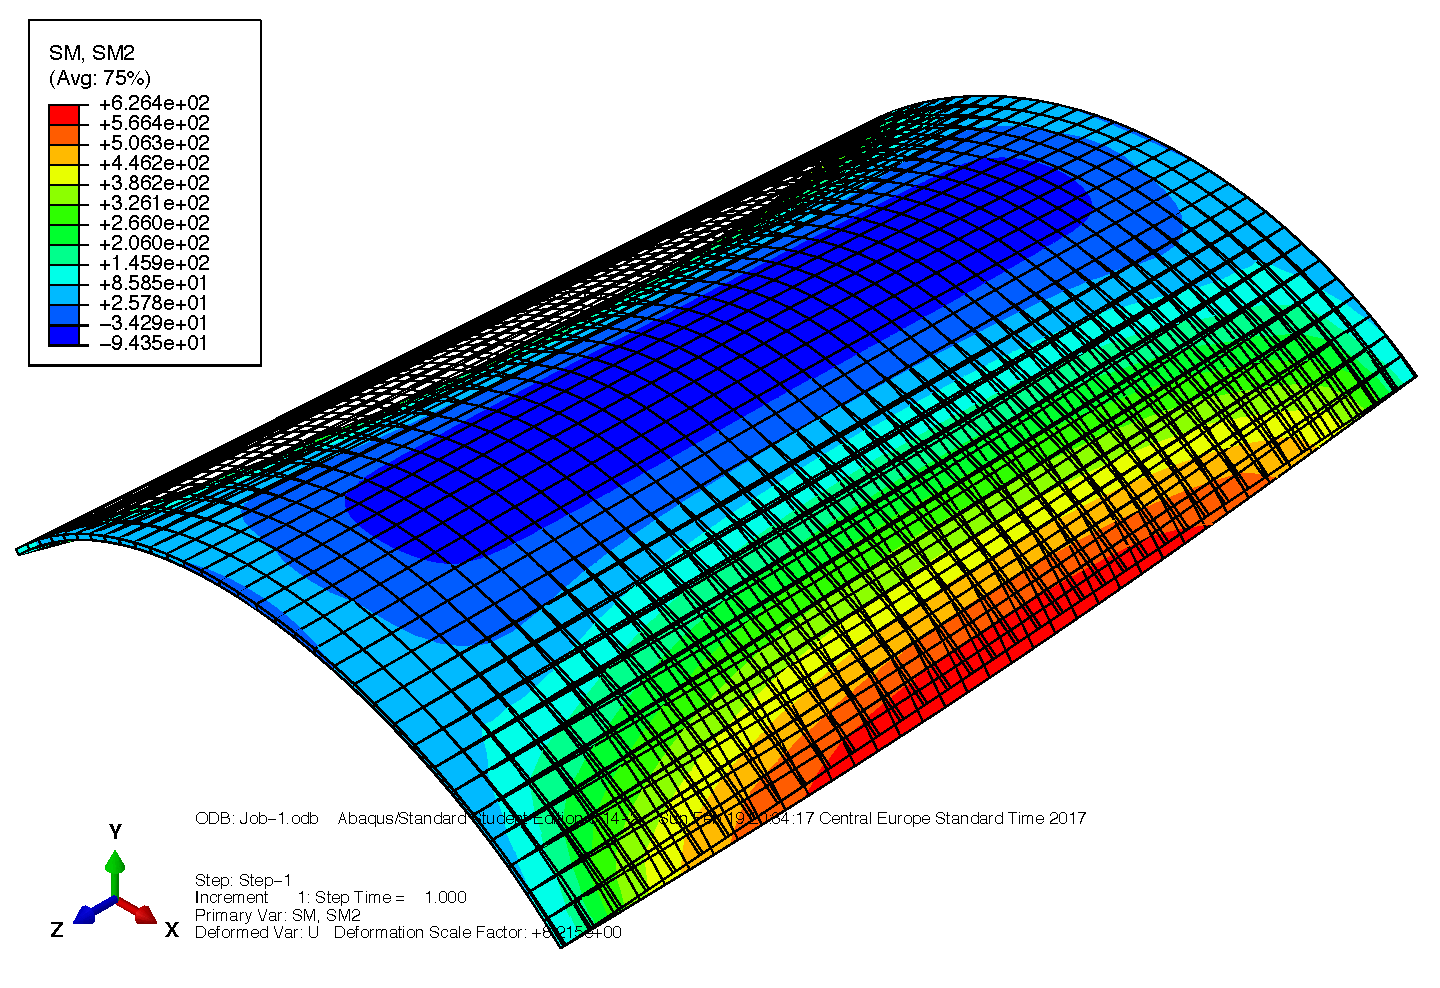
\includegraphics[scale=0.50]{figs/boveda2017-5}
	}
\author{%José M.ª Goicolea, Juan J. Arribas\\
        {\small\sc 
	Grupo de Mecánica Computacional, ETSICCP, UPM}}
\date{22-23 de febrero de 2023}


\begin{document}

\pagestyle{fancy}
\lhead[\fancyplain{}{\thepage}]{\fancyplain{}{\rightmark}}
\rhead[\fancyplain{}{\leftmark}]{\fancyplain{}{\thepage}}
\cfoot[\fancyplain{\thepage}{}]{\fancyplain{\thepage}{}}

%% \renewcommand{\chaptermark}[1]{\markboth{\sf\chaptername\ 
%%                                          \thechapter. \uppercase{#1}}{}}
\renewcommand{\sectionmark}[1]{\markright{\sf Aptdo.\ \thesection. #1}{}}

%\part{Métodos Generales de la Dinámica}
%\contentsline{part}{Métodos Generales de la Dinámica}{}
%\addcontentsline{toc}{part}{Métodos Generales de la Dinámica}
%\markboth{\sl Capítulo 1. Principios de la Mecánica.}{}

\maketitle

\tableofcontents

\addtocontents{toc}{\protect\hrule}

\section{Definición del problema}
\label{sec:problema}
Se considera una cubierta en forma de bóveda cilíndrica tendiendo un arco de $80^{\circ}$ (figura \ref{fig:esquema}). El material es elástico con módulo de Young $E=432\,\text{MPa}$ y coeficiente de Poisson $\nu=0$.
Las dimensiones son $R=25$ m, $L=50$ m, con espesor $t=0.25$ m.
\begin{figure}[!ht]
\centering
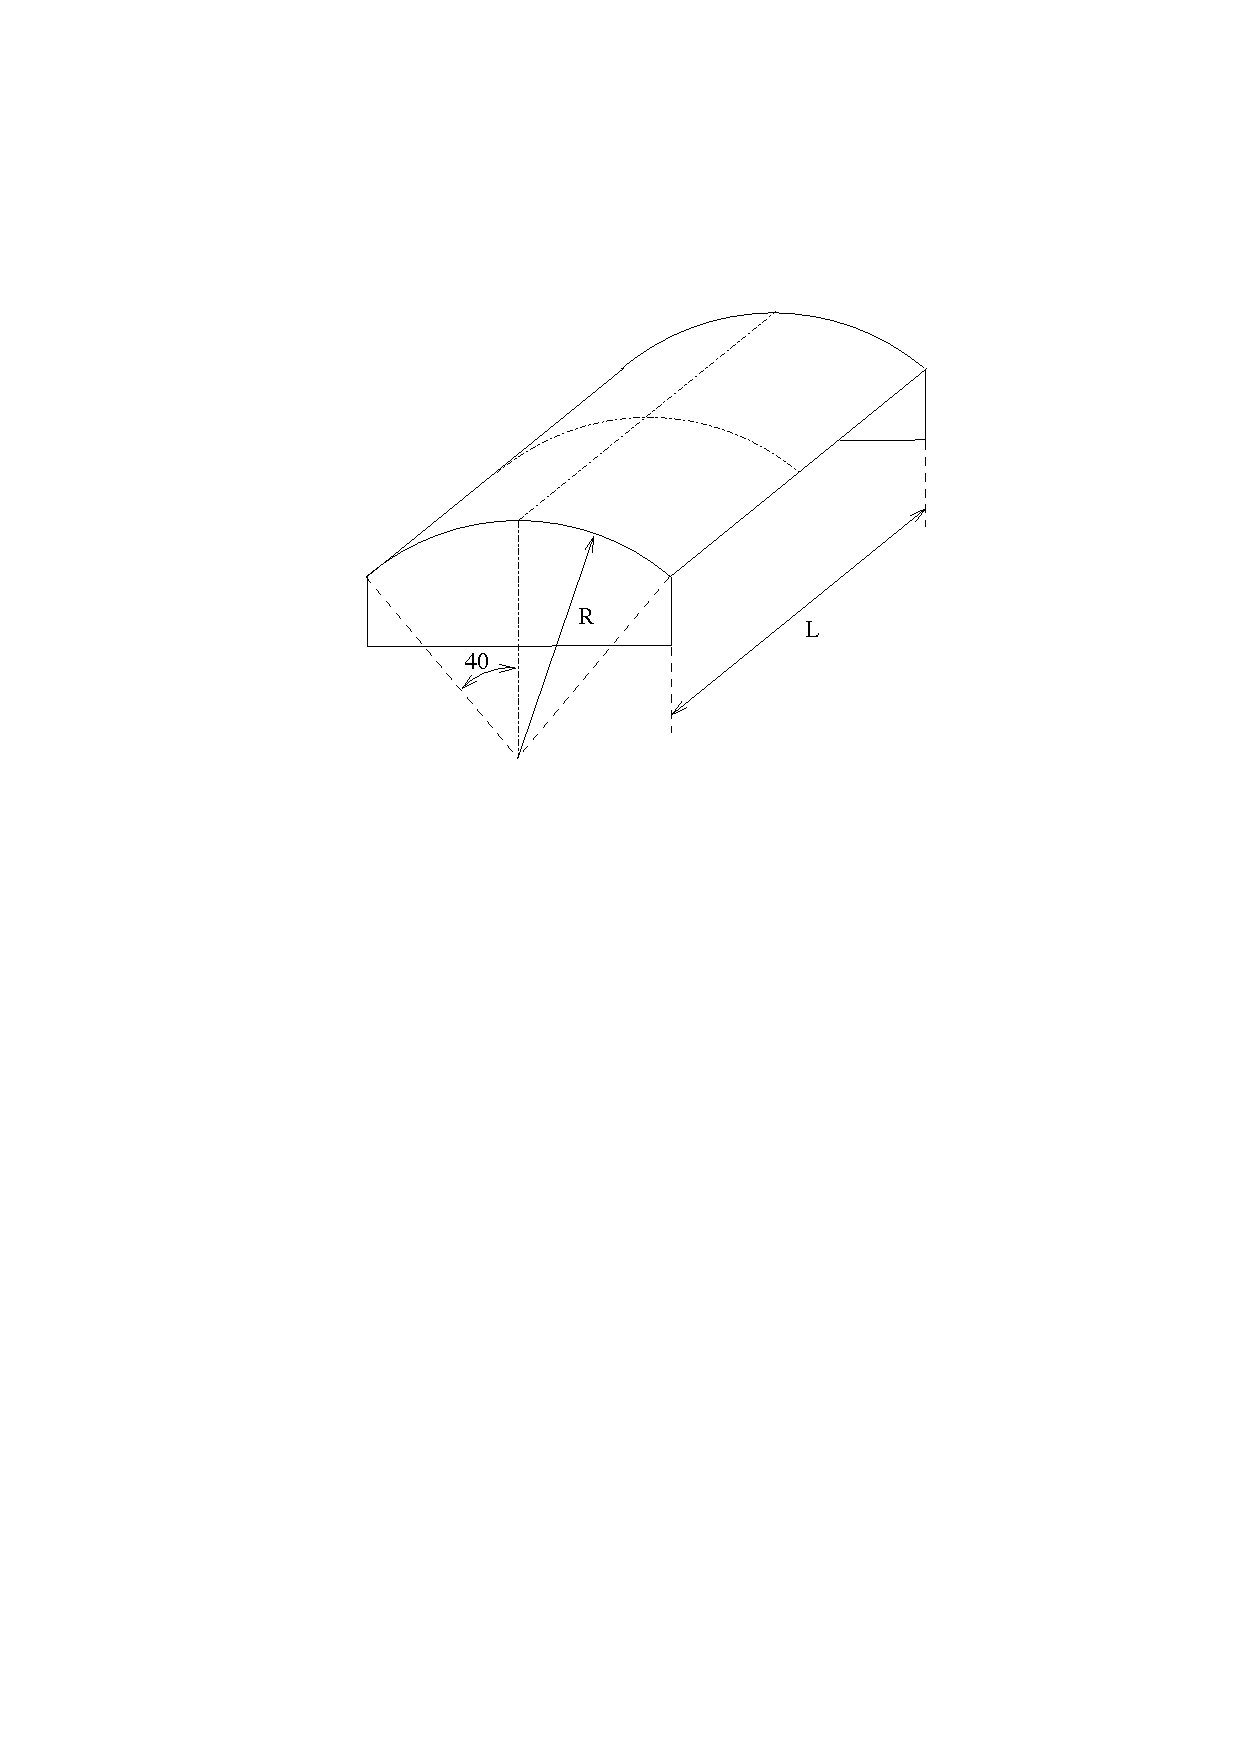
\includegraphics[width=0.5\textwidth]{figs/boveda_scordelis-lo}
\caption{Definición esquemática de la bóveda cilíndrica. }
\label{fig:esquema}
\end{figure}

Los dos extremos curvos están simplemente apoyados sobre diafragmas rígidos, de forma que los desplazamientos en dirección vertical y transversal están impedidos, mientras que el desplazamiento longitudinal es libre. 
Los bordes laterales rectos están libres, sin apoyar.
El conjunto está sometido a su propio peso, siendo el peso específico del material $\gamma=360\,\text{N/m}^{3}$.

Se pide:
\begin{enumerate}
\item
Resolver el problema con elementos lámina de 4 nodos, integración reducida y 5 gdl por nodo (S4R5).
Se tendrá en cuenta las simetrías existentes en la estructura, empleando una discretización de $16\times 16$ elementos para el modelo calculado. 
\item
Asimismo, aunque a priori no parezca la solución ideal, resolver con elementos sólidos con igual número de elementos en la superficie y un elemento tan solo en el espesor. 
Se obtendrá la solución con elementos sólidos hexaédricos de 8 nodos con integración completa (C3D8), con integración reducida (C3D8R) y con modos incompatibles (C3D8I).
\item
Se desea obtener como resultado del cálculo los desplazamientos en el borde libre y en el borde superior de la bóveda, así como en la sección central. 
Asimismo los esfuerzos de momentos flectores en dicha sección central, y las reacciones en los diafragmas.
\end{enumerate}

\textsc{Nota:} Se trata de un ejemplo clásico de prueba para elementos lámina propuesto por A. C. Scordelis y K. S. Lo, \emph{Computer analysis of cylindrical shells}; J. Amer. Concr. Inst 61, pp. 539-561 (1969).
El resultado de referencia que se puede considerar \emph{``exacto''}, para el desplazamiento vertical en el medio del borde libre, es $0.3024$ m.


\section{Modelo con elementos lámina}
\label{sec:guia}

\subsection{Módulo \texttt{Part}}

En primer lugar, se ejecuta \emph{Abaqus CAE} para crear un modelo nuevo. Para crear el modelo conviene obtener previamente algunos valores numéricos de coordenadas, que se pueden calcular como se indica en la figura \ref{fig:python}, mediante el intérprete de Python en el recuadro inferior de  la ventana.
\begin{figure}[h!tbp]
\begin{center}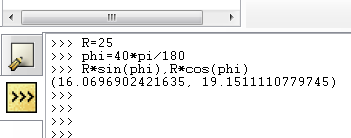
\includegraphics[scale=0.5]{capturas/01-python-calculos-aux.png}\end{center}
\caption{Cálculos auxiliares de coordenadas}
\label{fig:python}
\end{figure}

Se entra en el módulo \texttt{part}, activando el icono de crear una nueva parte, que se define como 3D, deformable, shell por extrusión (figura \ref{fig:arco}(a)).

El modelo se definirá empleando solo $1/4$ de la bóveda, haciendo uso de las simetrías longitudinal y transversal.
En primer lugar se define la directriz circular del arco transversal en el plano $xy$, mediante el icono de la utilidad de arco de circunferencia con centro y 2 puntos (figura \ref{fig:arco}(b)). El centro de la circunferencia se sitúa en $(0,0)$ y a continuación se dan las coordenadas de los dos extremos del arco, para $\phi=0$ y $\phi=40^{\circ}$. 
Los puntos a definir son $(0,R)$ y $(R\sin\phi, R\cos\phi)$, que habremos calculado antes numéricamente, y se escriben en la ventana de coordenadas (figura \ref{fig:arco}(c)).
Se recuerda que debe emplearse el punto como separador decimal, no la coma.
Una vez introducido el último punto, en este caso el tercero, pulsar el botón con el aspa roja (figura \ref{fig:arco}(c)).

\emph{OJO}: hay que tener cuidado cuando se está generando el arco para que lo haga en el sentido deseado de la circunferencia; para ello el cursor del ratón deberá estar posicionado en la zona deseada cuando se introducen las coordenadas.
\begin{figure}[h!tp]
\centering
\subfigure[Crear nueva parte]{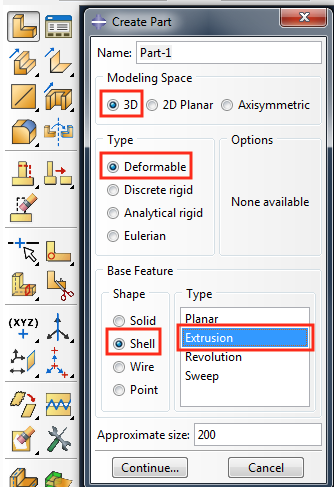
\includegraphics[scale=0.4]{capturas/02-partx.png}}
\subfigure[Arco con centro y 2 puntos]{\parbox[t]{0.30\textwidth}{%
\centering
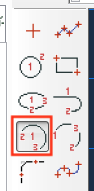
\includegraphics[scale=0.4]{capturas/03-partx.png}%
}}
\subfigure[Introducción de coordenadas]{
%\includegraphics[scale=0.4]{figs/01_end-coordinate-input-x}

\includegraphics[scale=0.4]{capturas/04-part}
}
\caption{Creación de la geometría del arco}
\label{fig:arco}
\end{figure}

Una vez creado el arco se culmina con el botón ``Done'' (figura \ref{fig:extru}(a)) y se realiza la extrusión de $L/2=25$ (figura \ref{fig:extru}(b)).
Por esta operación obtendremos una lámina curva desde el plano $z=0$ hasta el plano $z=L/2$.
Los planos verticales $z=0$ y $x=0$ serán los considerados como planos de simetría.
Se obtiene el resultado mostrado en la figura \ref{fig:extru1}.
\begin{figure}[h!tp]
\centering
\subfigure[seleccionar arco]{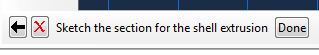
\includegraphics[scale=0.5]{capturas/05-part.png}}
\subfigure[definir extrusión]{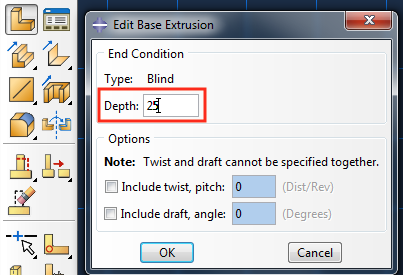
\includegraphics[scale=0.5]{capturas/06-partx.png}}
\caption{Bóveda como extrusión del arco, entre $z=0$ y $z=L/2=25$.}
\label{fig:extru}
\end{figure}
\begin{figure}[h!tp]
\centering
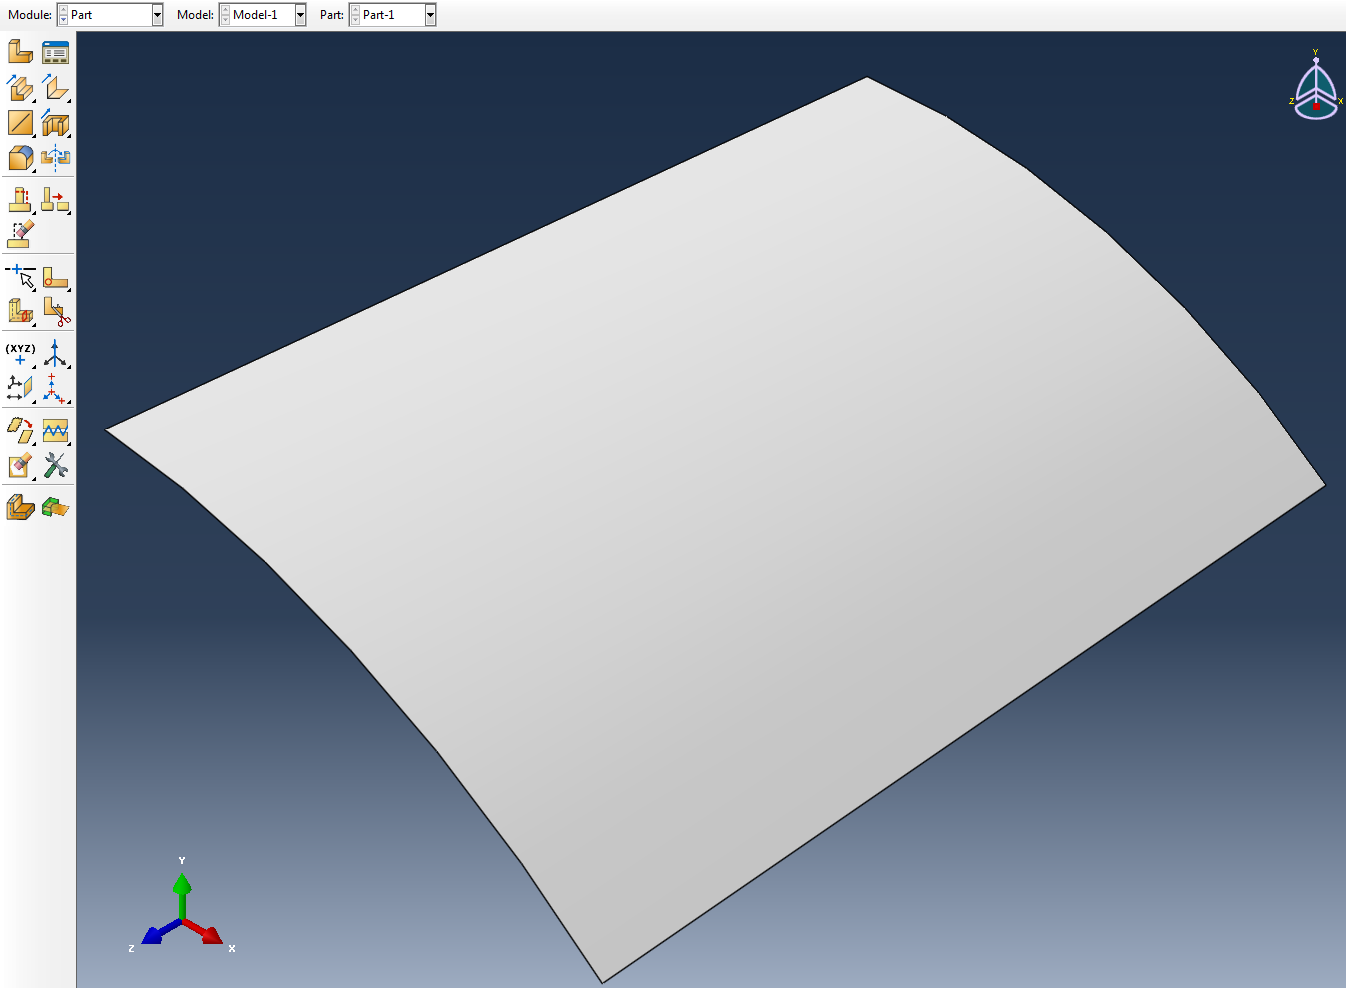
\includegraphics[scale=0.35]{capturas/07-part.png}
\caption{Geometría generada de la bóveda cilíndrica como extrusión del arco, entre $z=0$ (parte posterior de la figura) y $z=L/2=25$ (parte anterior).}
\label{fig:extru1}
\end{figure}
\clearpage

\subsection{Módulo \texttt{Property}}

Se activa el icono para crear material nuevo (figura \ref{fig:propmat}(a)),
se selecciona el material elástico lineal y se introducen las propiedades $E=432\cdot 10^{6}\,\text{Pa}, \nu=0$
(figura \ref{fig:propmat}(b)).
\begin{figure}[h!tp]
\centering
\subfigure[icono]{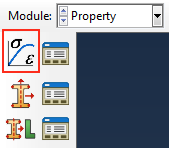
\includegraphics[scale=0.50]{capturas/08-propertyx.png}}
\subfigure[tipo de material y propiedades]{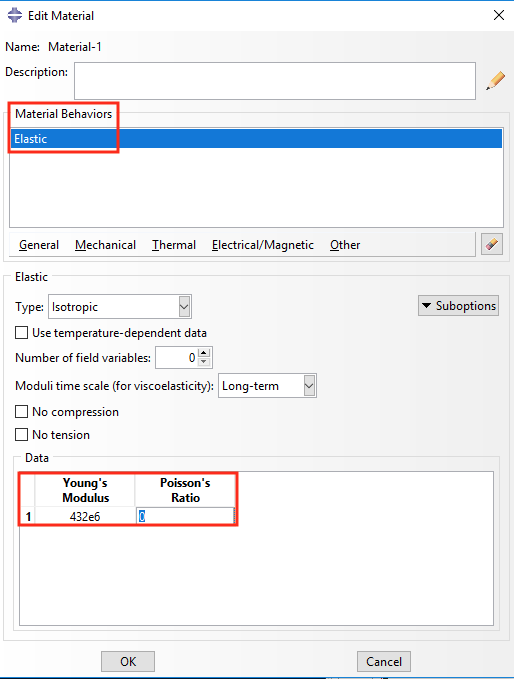
\includegraphics[scale=0.50]{capturas/09-property-x.png}}
\caption{Crear material nuevo}
\label{fig:propmat}
\end{figure}

A continuación se crea una \emph{``sección''}, en la que se definen sus propiedades, en este caso el espesor de la lámina $(0.25\,\text{m})$ y la opción \emph{Before analysis} (figura \ref{fig:section-properties}). 
Esta opción implica el cálculo mediante resultantes seccionales (es decir, momentos flectores, cortantes, axiles\ldots), en lugar de integrar las tensiones numéricamente en una serie de puntos del espesor.
Esto último que podría ser necesario en un modelo de material no lineal, lo que no es el caso.
A continuación se asigna la sección a la parte creada (figura \ref{fig:section-assign}).
\begin{figure}[h!tp]
\centering
\subfigure[tipo]{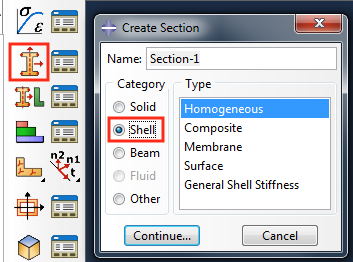
\includegraphics[scale=0.4]{capturas/10-property-x.png}}
\subfigure[datos]{
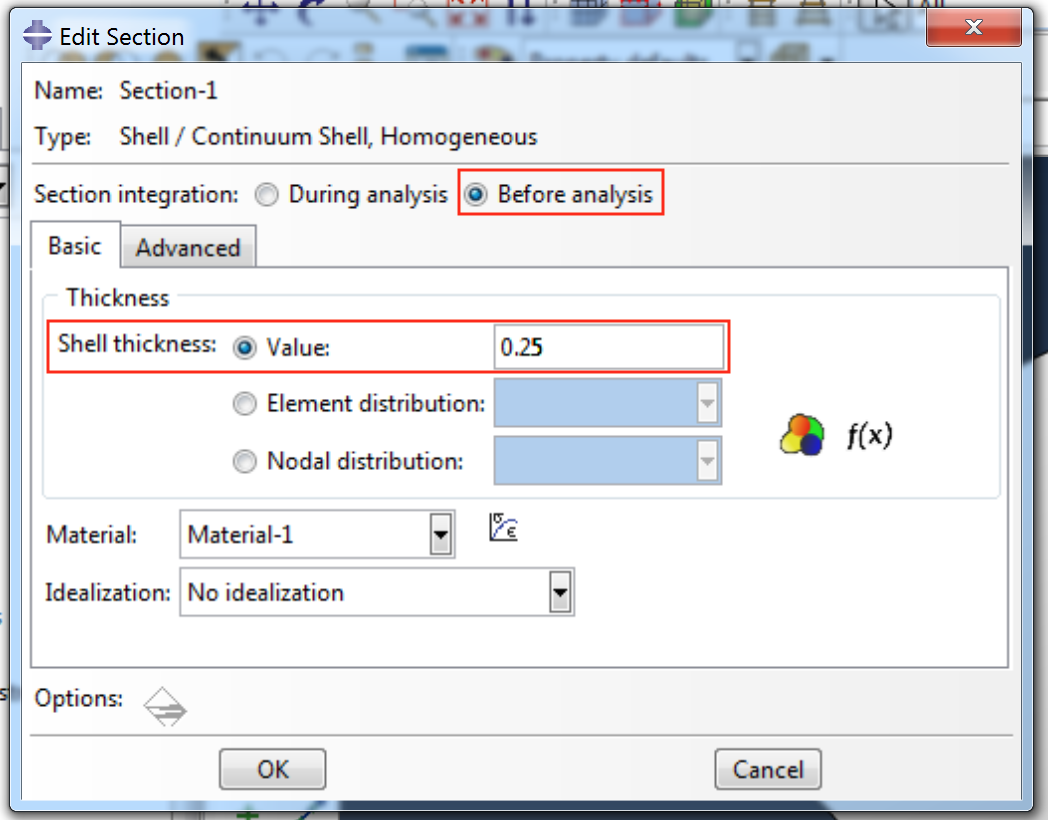
\includegraphics[scale=0.4]{capturas/02a_shell-thickness-type-selection-x}
%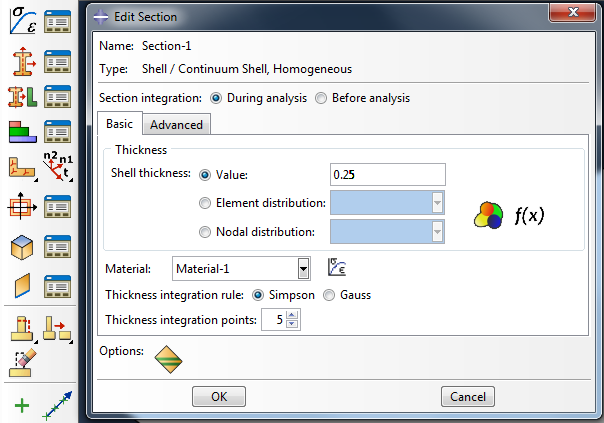
\includegraphics[scale=0.4]{capturas/11-property.png}
}
\caption{Definición y propiedades de la sección}
\label{fig:section-properties}
\end{figure}

\begin{figure}[h!tp]
\centering
\subfigure[asignar sección]{\parbox[t]{0.2\textwidth}{%
\centering

\includegraphics[scale=0.6]{capturas/03a_assign-section-icon}%
}}
\subfigure[seleccionar parte]{%
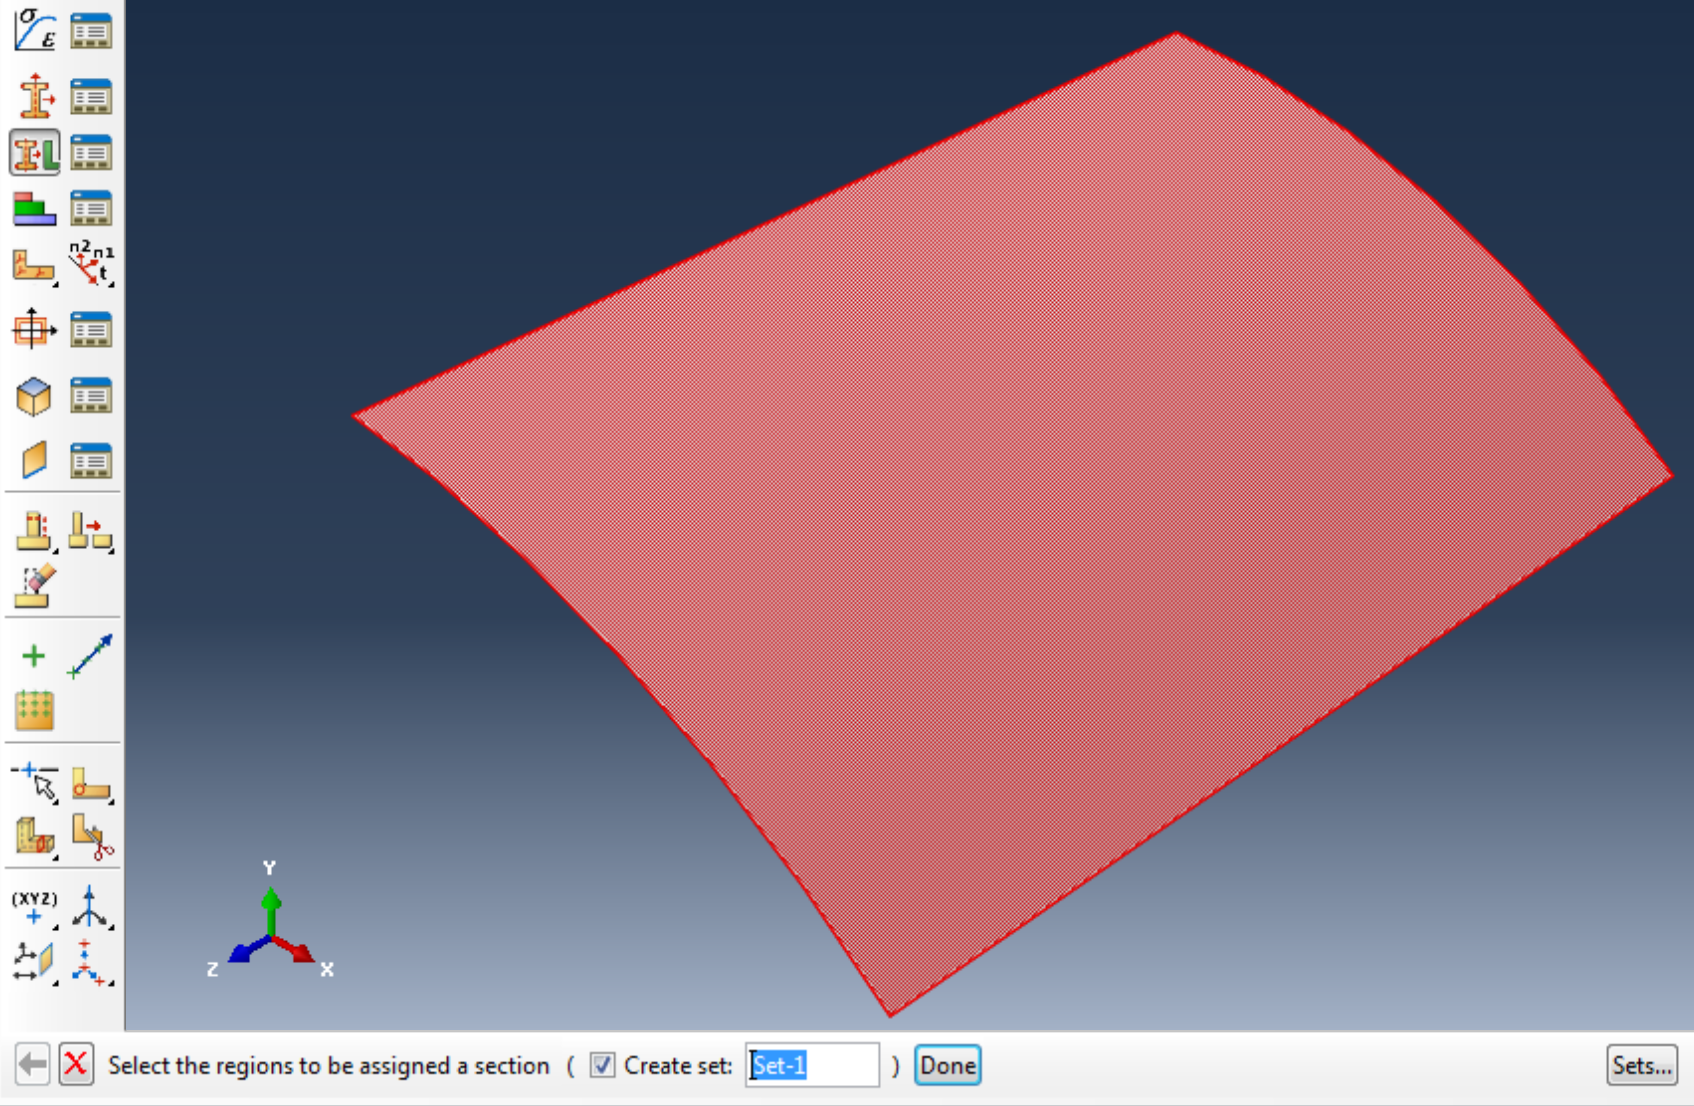
\includegraphics[scale=0.4]{capturas/04a_select-region-to-assign-section}
%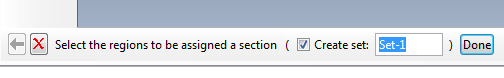
\includegraphics[scale=0.4]{capturas/12-property.png}
}
\subfigure[asignación]{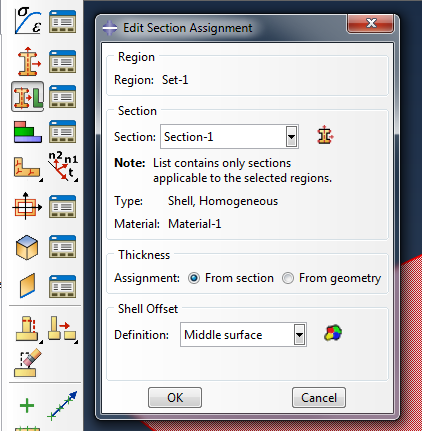
\includegraphics[scale=0.4]{capturas/13-property.png}}
\subfigure[parte asignada]{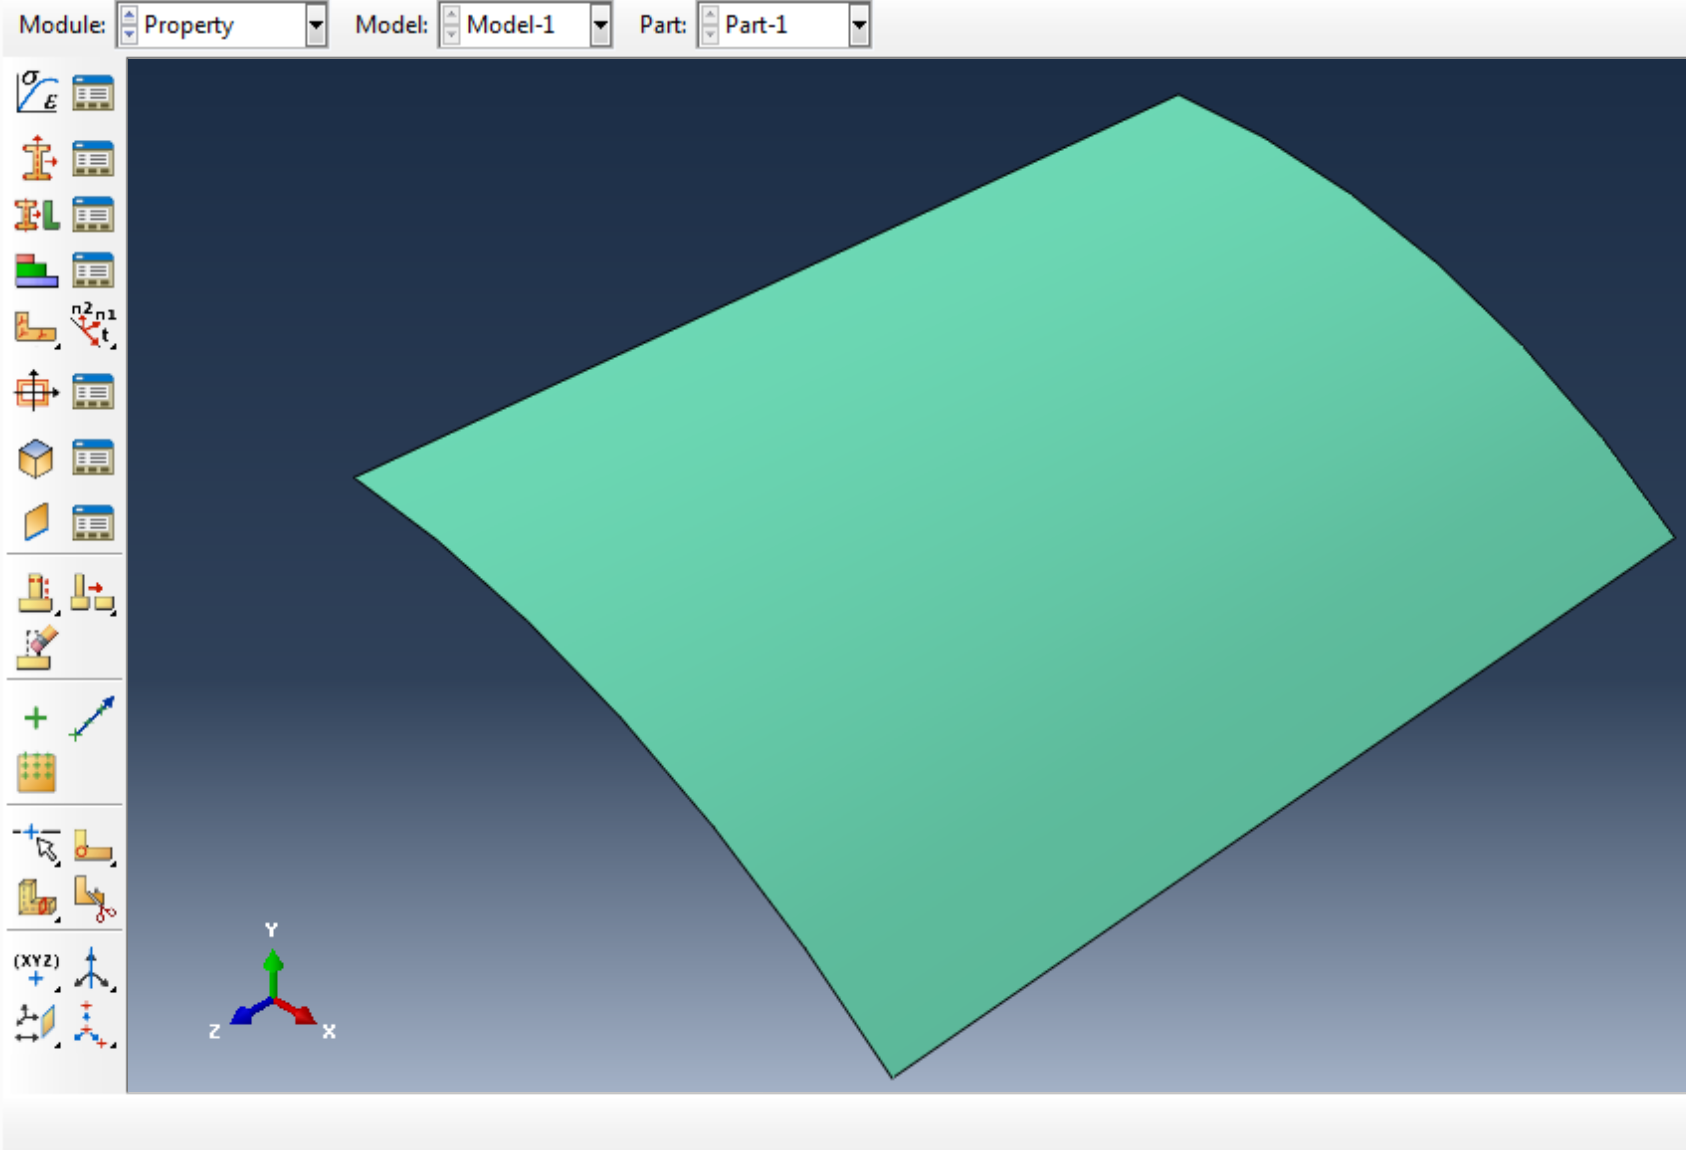
\includegraphics[scale=0.3]{capturas/05a_section-assigned}}
\caption{Asignación de la sección}
\label{fig:section-assign}
\end{figure}
\clearpage

\subsection{Módulo \texttt{Assembly}}

En este módulo tan solo hay que crear una ``instancia'' a partir de la parte, mediante las opciones por defecto:
\begin{figure}[h!tp]
\centering
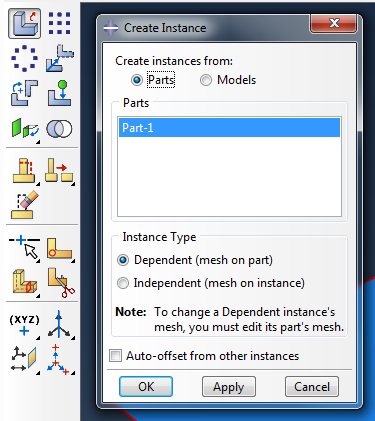
\includegraphics[scale=0.4]{capturas/14-assembly.png}
\caption{Assembly: crea una instancia de la parte}
\label{fig:assembly}
\end{figure}

\subsection{Módulo \texttt{Step}}

Se crea un ``step'' para el procedimiento de cálculo ``Static, general''. Se toman las opciones por defecto (figura \ref{fig:step}). 
Se edita en ``field output'' el conjunto de variables para agregar los esfuerzos seccionales SF (esfuerzos de membrana y de flexión de la lámina), como se indica en la
figura \ref{fig:field-output}.
\begin{figure}[h!tp]
\centering
\subfigure[Creación]{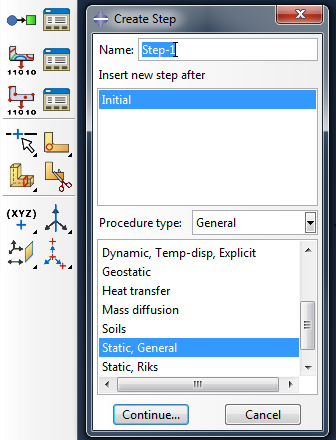
\includegraphics[scale=0.4]{capturas/15-step.png}}
\subfigure[Definición]{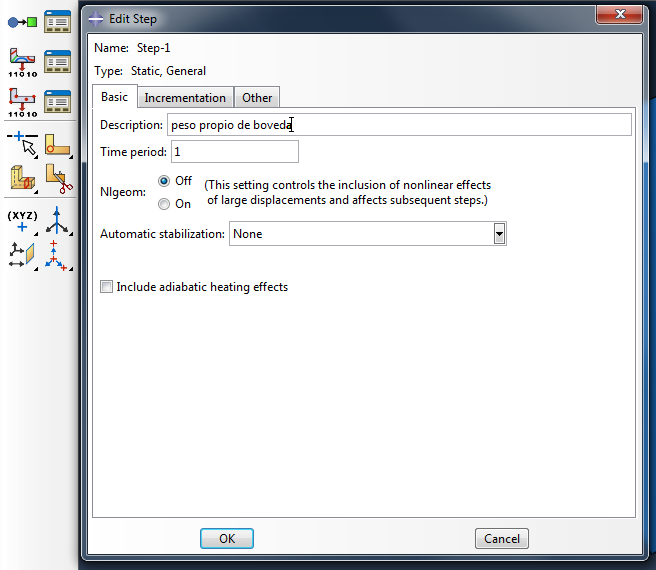
\includegraphics[scale=0.4]{capturas/16-step.png}}
\caption{Crear y definir el ``step''}
\label{fig:step}
\end{figure}
\begin{figure}[h!tp]
\centering
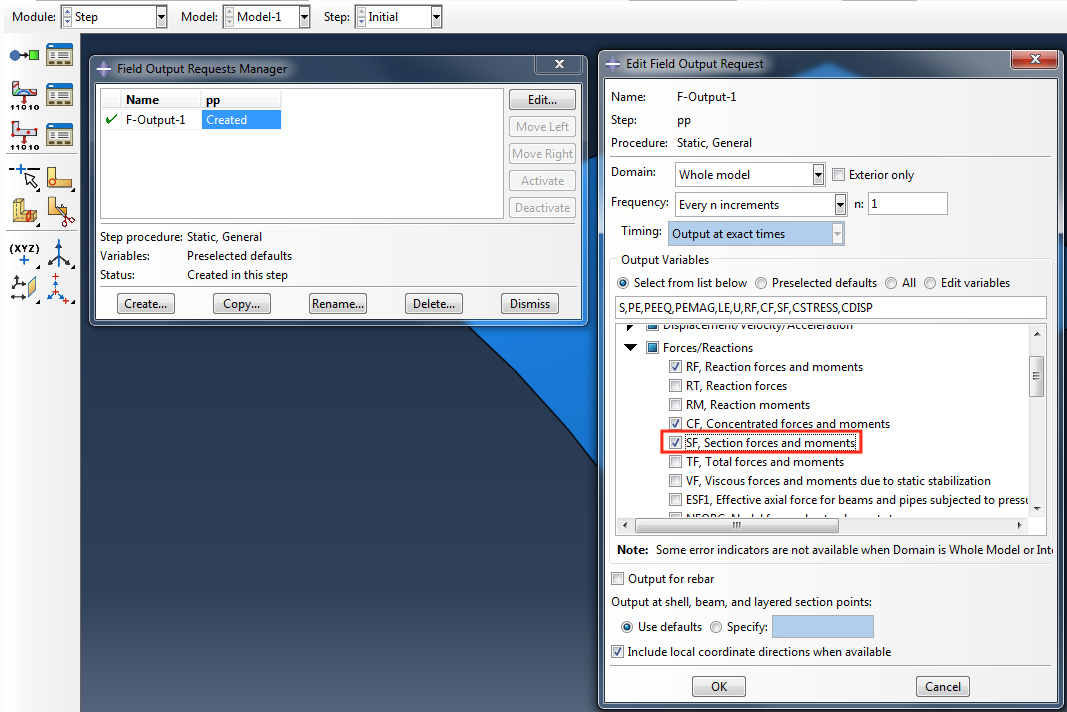
\includegraphics[scale=0.4]{capturas/16a-step-x.png}
\caption{Modificación del ``field output''}
\label{fig:field-output}
\end{figure}
\clearpage

\subsection{Módulo \texttt{Load}}


En el módulo \texttt{Load} se definirán tanto las cargas aplicadas como las condiciones de contorno. 
En primer lugar las cargas, que son únicamente las de peso propio, mediante ``Body force'', a la que se da un valor $q_{y}=-360\,\text{N/m}^{3}$ (figura \ref{fig:pp}).
El resultado final se visualiza en la figura \ref{fig:pp}(d)
\begin{figure}[h!tp]
\centering
\subfigure[selecciona ``Body force'']{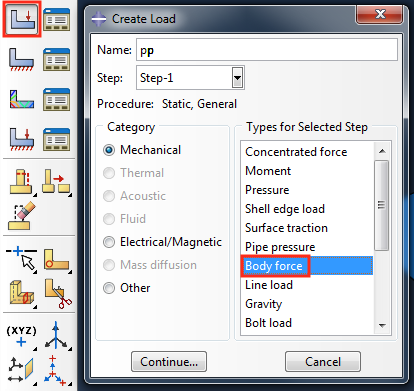
\includegraphics[scale=0.5]{capturas/17-load-x.png}}
\subfigure[selecciona el cuerpo]{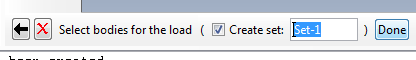
\includegraphics[scale=0.5]{capturas/18-load.png}}
\subfigure[valor de la carga]{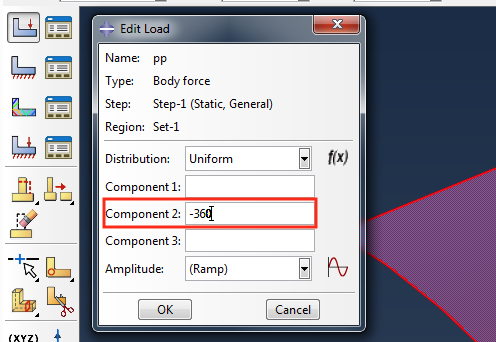
\includegraphics[scale=0.4]{capturas/19-load-x.png}}
\subfigure[aspecto final]{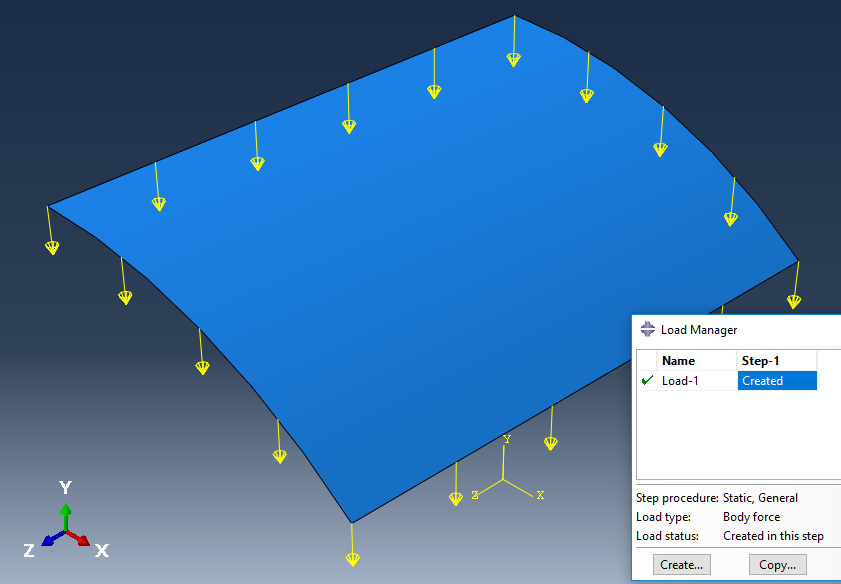
\includegraphics[scale=0.3]{capturas/20-bodyforce-shell.png}}
\caption{Definición de las cargas de peso propio}
\label{fig:pp}
\end{figure}
%\clearpage

A continuación se imponen las condiciones de contorno, primero las que corresponden a los dos planos de simetría.
Se abre el ``manager'' de condiciones de contorno y se crea la condición adecuada en el borde $x=0$, condiciones ``Symmetry/Antisymmetry'' del tipo ``XSYMM'', una vez seleccionado con el ratón el borde adecuado (ojo, !`hay que tener cuidado para no seleccionar más que ese borde!)
(figura \ref{fig:xsymm}).
\begin{figure}[h!tp]
\centering
\subfigure[Seleccionar borde y condición XSYMM]{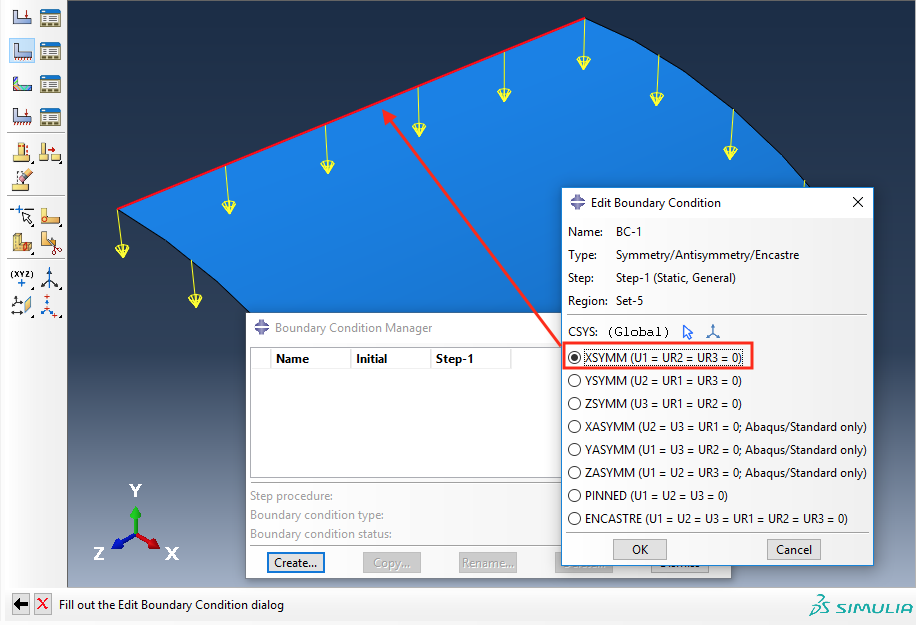
\includegraphics[scale=0.25]{capturas/25-load-x.png}}
\subfigure[Simetría XSYMM creada]{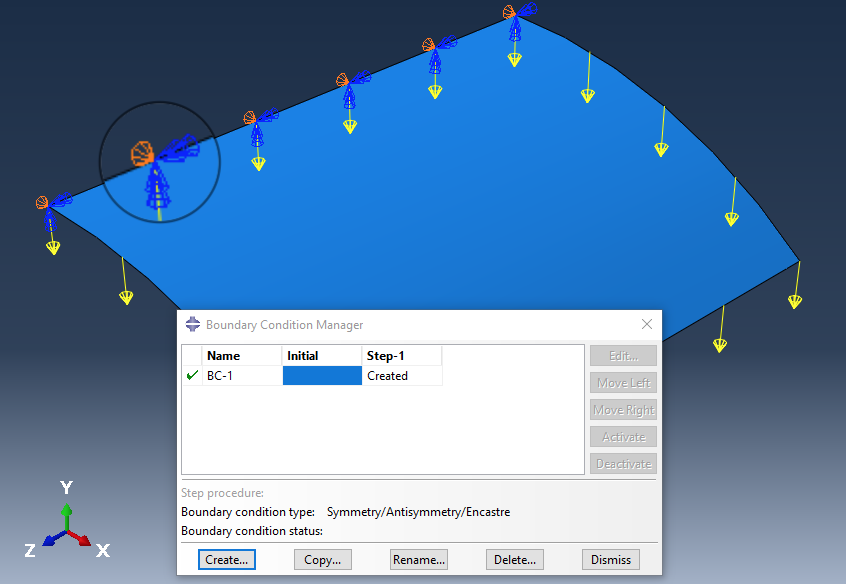
\includegraphics[scale=0.25]{capturas/26-load-x.png}}
\caption{Condiciones de contorno de simetría ``XSYMM''}
\label{fig:xsymm}
\end{figure}

Se establece ahora la simetría por el plano $z=0$, es decir en el borde posterior del modelo, imponiendo las condiciones correspondientes ``ZSYMM''
(figura \ref{fig:zsymm})
\begin{figure}[h!tp]
\centering
\subfigure[Seleccionar borde y condición ZSYMM]{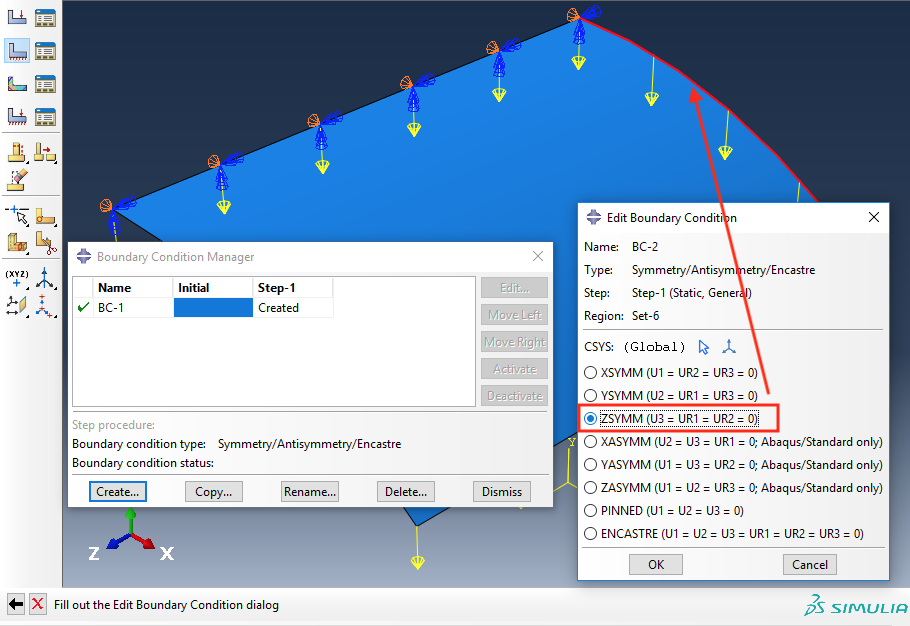
\includegraphics[scale=0.25]{capturas/27a-load-x.png}}
\subfigure[Simetría ZSYMM creada]{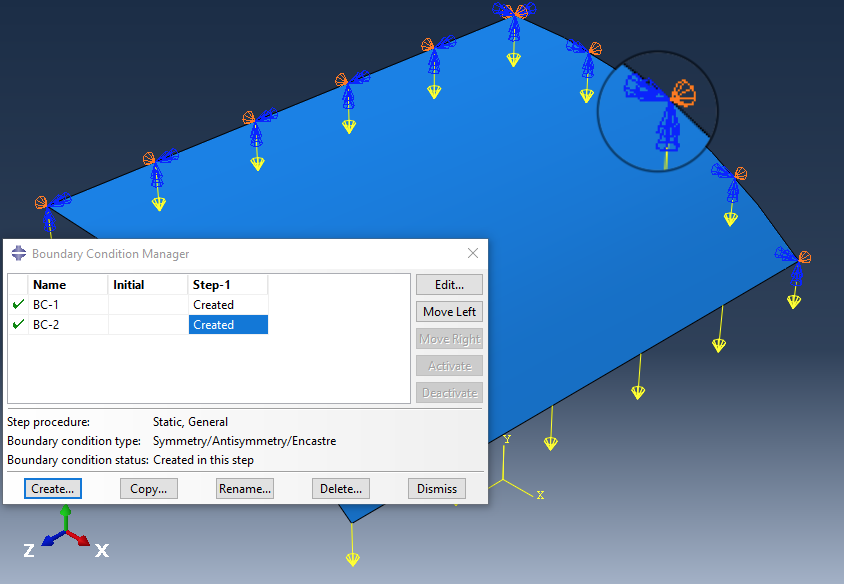
\includegraphics[scale=0.25]{capturas/27b-load-x.png}}
\caption{Condiciones de contorno de simetría ``ZSYMM'' en borde posterior}
\label{fig:zsymm}
\end{figure}

Por último, en el borde anterior $z=L/2$, se crea una condición de contorno para imponer el apoyo fijo, mediante condiciones del tipo ``Displacement/rotation'', fijándose únicamente los grados de libertad $u_{x}, u_{y}$ (U1 y U2 en Abaqus):
(figura~\ref{fig:apoyo}(a)).
Al final, el conjunto de cargas y condiciones de contorno definidas se muestran en la figura~\ref{fig:apoyo}(b).
\begin{figure}[h!tp]
\centering
\subfigure[Apoyo en borde anterior]{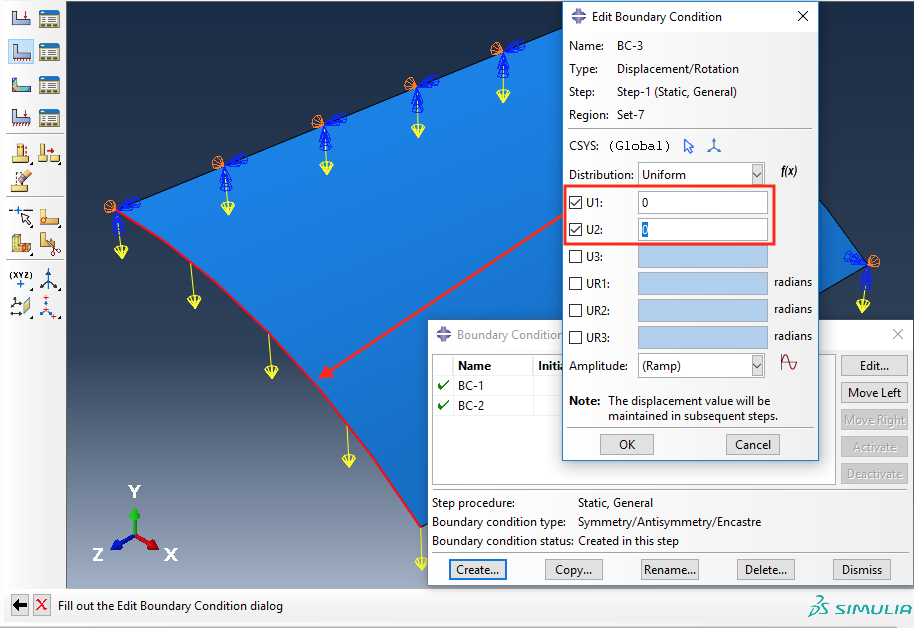
\includegraphics[scale=0.25]{capturas/28b-load-x.png}}
\subfigure[Apoyo y resto de condiciones]{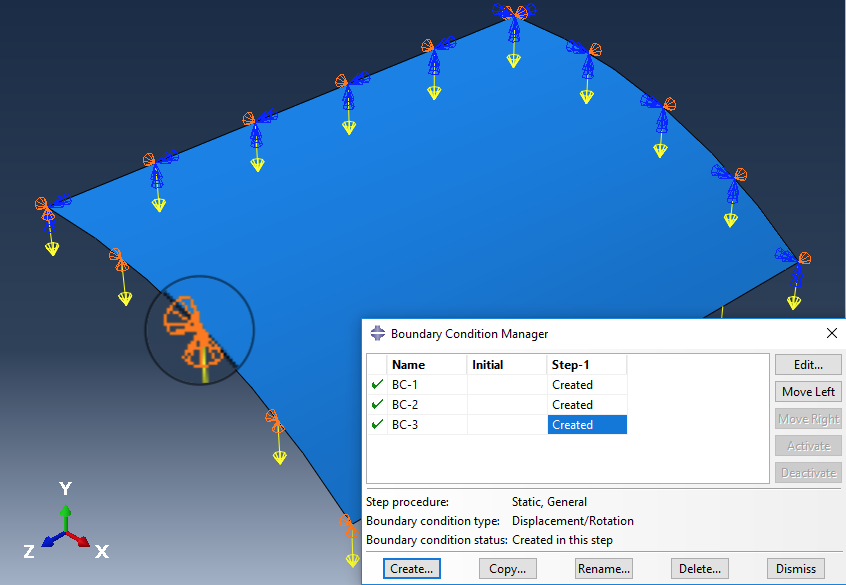
\includegraphics[scale=0.25]{capturas/28c-load-x.png}}
\caption{Condiciones de contorno en el apoyo en el borde anterior}
\label{fig:apoyo}
\end{figure}
\clearpage

\subsection{Módulo \texttt{Mesh}}

%Within the \texttt{Mesh} module, start by selecting the part by expanding the tee of the model at the left side, and activating with the right button the icon \emph{``Mesh''}:
En el módulo mesh hay que comenzar por seleccionar la parte expandiendo el árbol del modelo / parte de la izquierda, y activando con el botón derecho el icono \emph{``Mesh''}:
Fig.~\ref{fig:mesh-part}.
%Open in the top menu bar \emph{Mesh} $\to$ \emph{Controls} and select ``Quad'' and ``Structured'', to generate s structured mesh of quadrilaterals 
Se abre en el menú superior \emph{Mesh} $\to$ \emph{Controls} y se selecciona ``Quad'' y ``Structured'', para generar una malla estructurada de cuadriláteros
(Fig. \ref{fig:mesh-controls}).
\begin{figure}[h!tp]
\parbox[t]{0.49\textwidth}{%
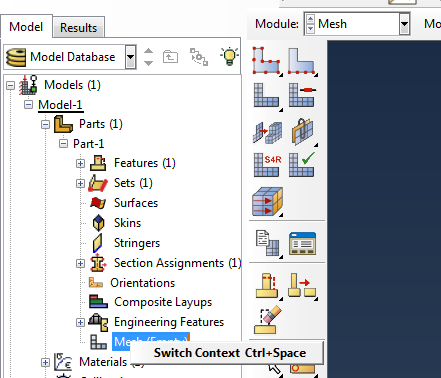
\includegraphics[width=0.5\textwidth]{capturas/29-mesh.png}
%\caption{Expanded model tree for mesh.}
\caption{Seleccionar en el menú desplegado del modelo para mallar.}
\label{fig:mesh-part}%
}\quad
\parbox[t]{0.49\textwidth}{%
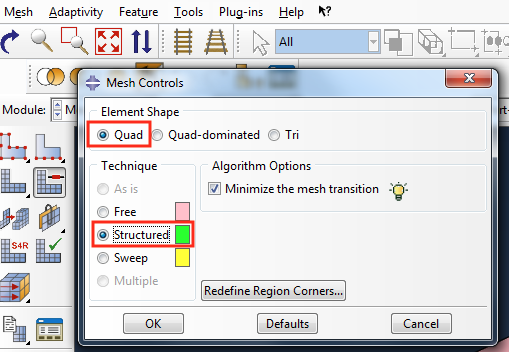
\includegraphics[width=0.5\textwidth]{capturas/30-mesh-x.png}
%\caption{Define options in ``Mesh controls''}
\caption{Definir opciones en ``Mesh controls''}
\label{fig:mesh-controls}%
}%
\end{figure}

%Following, open in the top bar the menu \emph{Mesh} $\to$ \emph{Element type} and select the options \emph{``Shell''}, \emph{``Membrane stress: Small''}, \emph{``Reduced integration''} which will correspond to element type S4R5
A continuación se abre en el menú superior \emph{Mesh} $\to$ \emph{Element type} y se seleccionan las opciones ``Shell'', ``Membrane strain: Small'', lo que dará lugar al elemento S4R5 
(Fig. \ref{fig:mesh-element}).
\begin{figure}[h!tp]
\centering
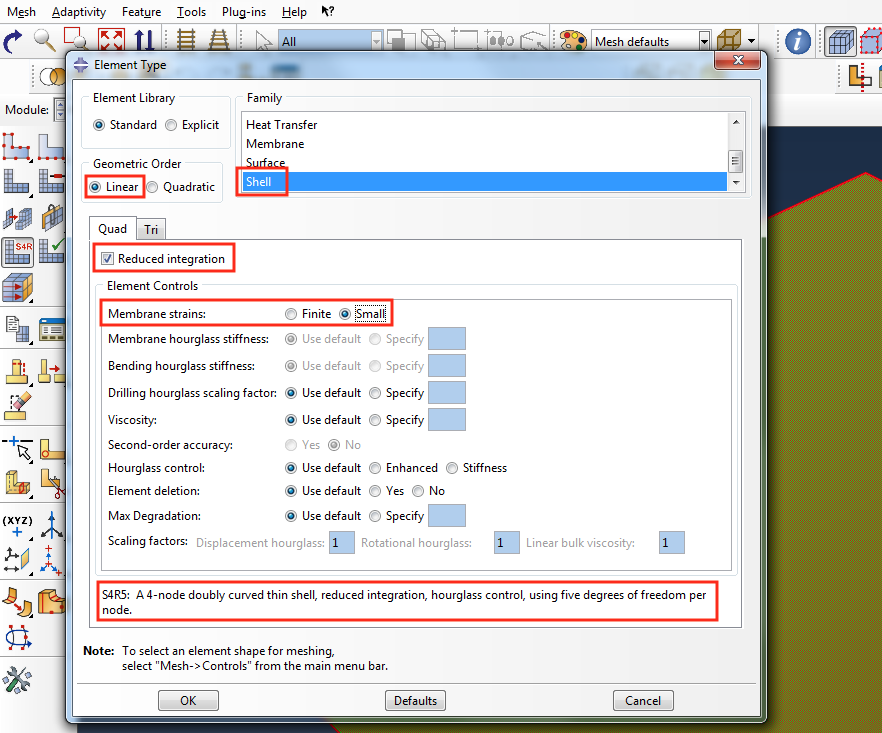
\includegraphics[scale=0.33]{capturas/31-mesh.png}
\caption{Seleccionar tipo de elemento en ``Mesh/element''}
\label{fig:mesh-element}%
\end{figure}

%Following the seeds for mesh generation are introduced, this will be done individually for each edge
Ahora se introducen las semillas para la generación de la malla, se seleccionan los bordes individuales, se activa la opción ``By number'' y se piden 16 elementos por borde. Esta operación hay que hacerla en dos bordes ortogonales, en los otros dos no es necesario
(figura \ref{fig:seeds}).
\begin{figure}[h!tp]
\centering
\subfigure[]{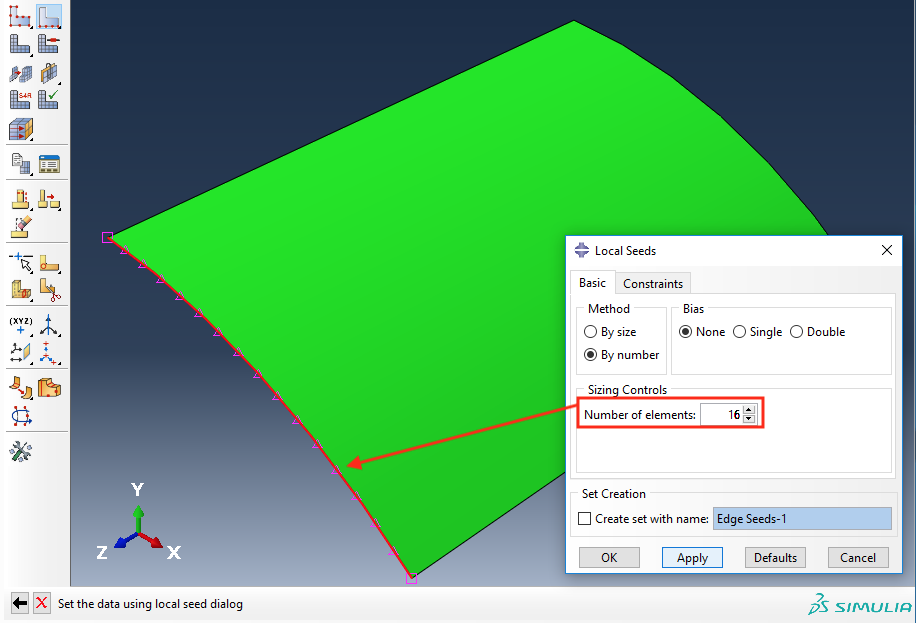
\includegraphics[scale=0.25]{capturas/33a-mesh-x.png}}
\subfigure[]{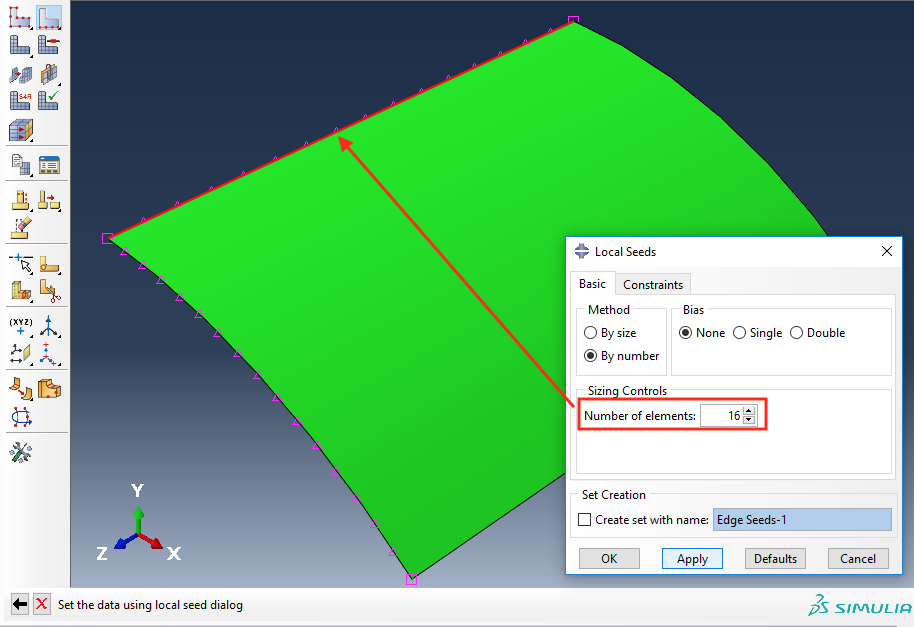
\includegraphics[scale=0.25]{capturas/33b-mesh-x.png}}
\caption{Definición de número de elementos (semillas) en cada borde}
\label{fig:seeds}
\end{figure}
Finalmente se malla la parte con el icono de mallado indicado en la figura~\ref{fig:mesh}, obteniéndose el resultado que se muestra.
\begin{figure}[h!tp]
\centering
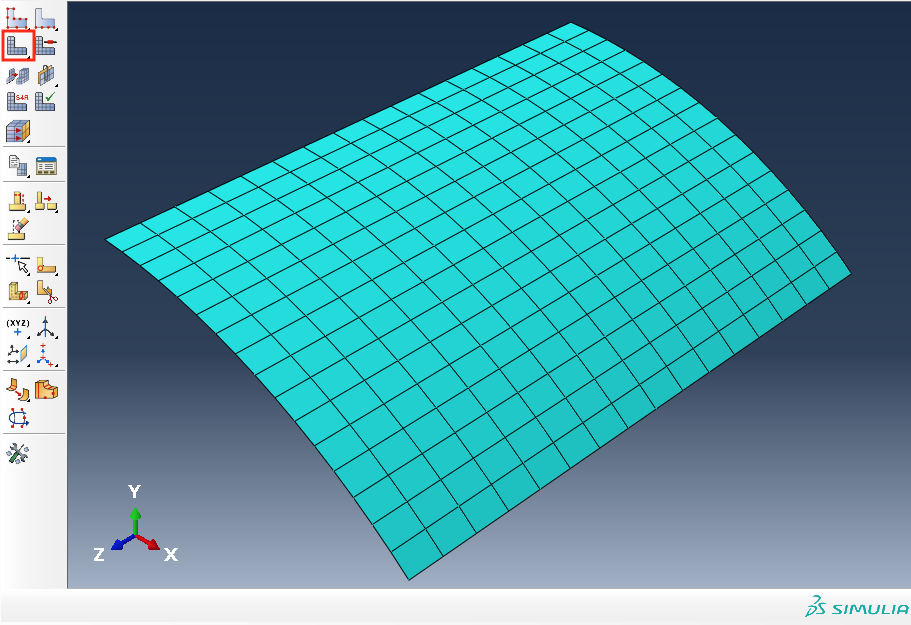
\includegraphics[scale=0.30]{capturas/36-mesh-x.png}
\caption{Mallado del cuerpo}
\label{fig:mesh}
\end{figure}
%\clearpage

\subsection{Módulo \texttt{Job}}

Una vez completado el modelo, se crea un ``Job'' con las opciones por defecto
(figura \ref{fig:job-create}).
\begin{figure}[h!tp]
\centering
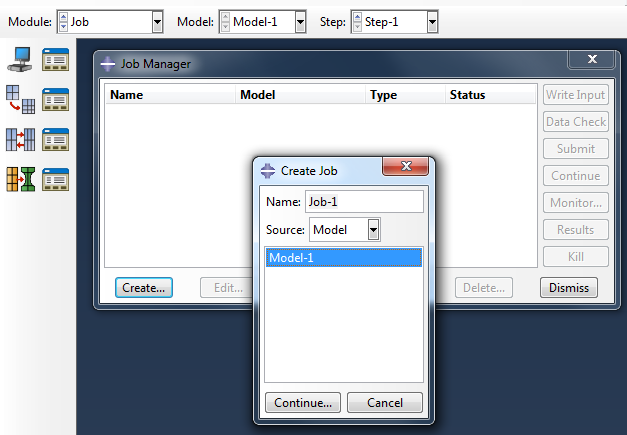
\includegraphics[scale=0.5]{capturas/37-job.png}
\caption{Creación del ``Job''}
\label{fig:job-create}
\end{figure}

Y se envía para calcular mediante ``Submit''. El \emph{Status} va cambiando de ``Submitted'' $\to$ ``Running'' $\to$ ``Completed''. 
(figura \ref{fig:job-submit})
\begin{figure}[h!tp]
\centering
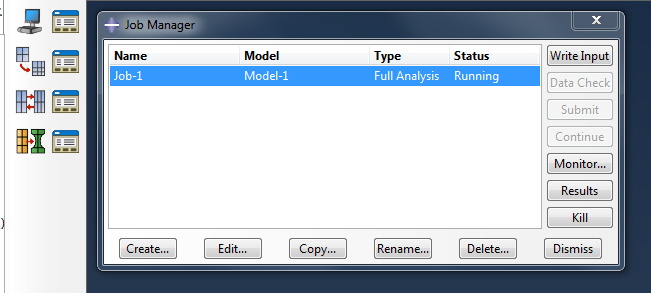
\includegraphics[scale=0.5]{capturas/38-job.png}
\caption{Envío del ``Job''}
\label{fig:job-submit}
\end{figure}
Si no hay mensaje de error el problema está acabado y se pasa al módulo de visualizar los resultados, como se muestra en la
figura \ref{fig:job-results}.
Se observa que la flecha en el punto medio del borde libre es muy próxima al valor de referencia  $u_{z}=-0.3024$ m.
% con la malla 16x16 resulta $u_{z}=-0.3043$ m

A menudo resulta conveniente representar el modelo completo con las partes simétricas que se han considerado implícitamente, representadas como imagen especular. 
Esto se puede obtener mediante las opciones en el menú ``View'' $\to$ ``ODB display options'', escogiendo en la pestaña ``Mirror / Patterns'' los \emph{Mirror planes} para $XY$ e $YZ$,
figura \ref{fig:job-results-symm}.
\begin{figure}[h!tp]
\centering
%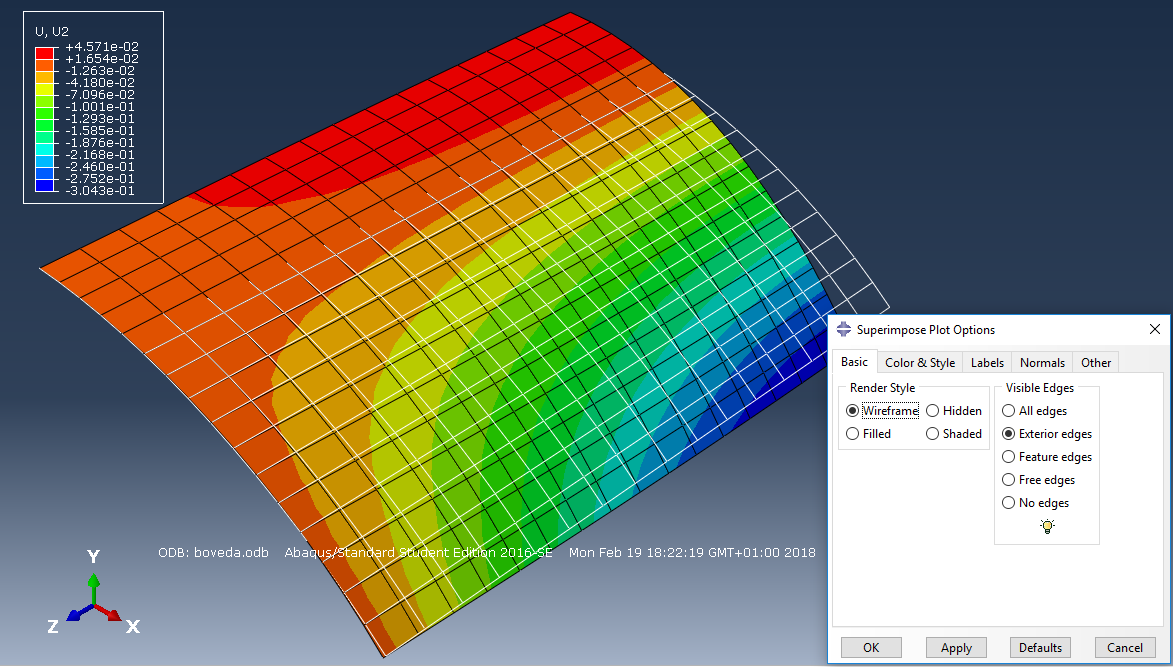
\includegraphics[scale=0.35]{capturas/39-results-U2.png}
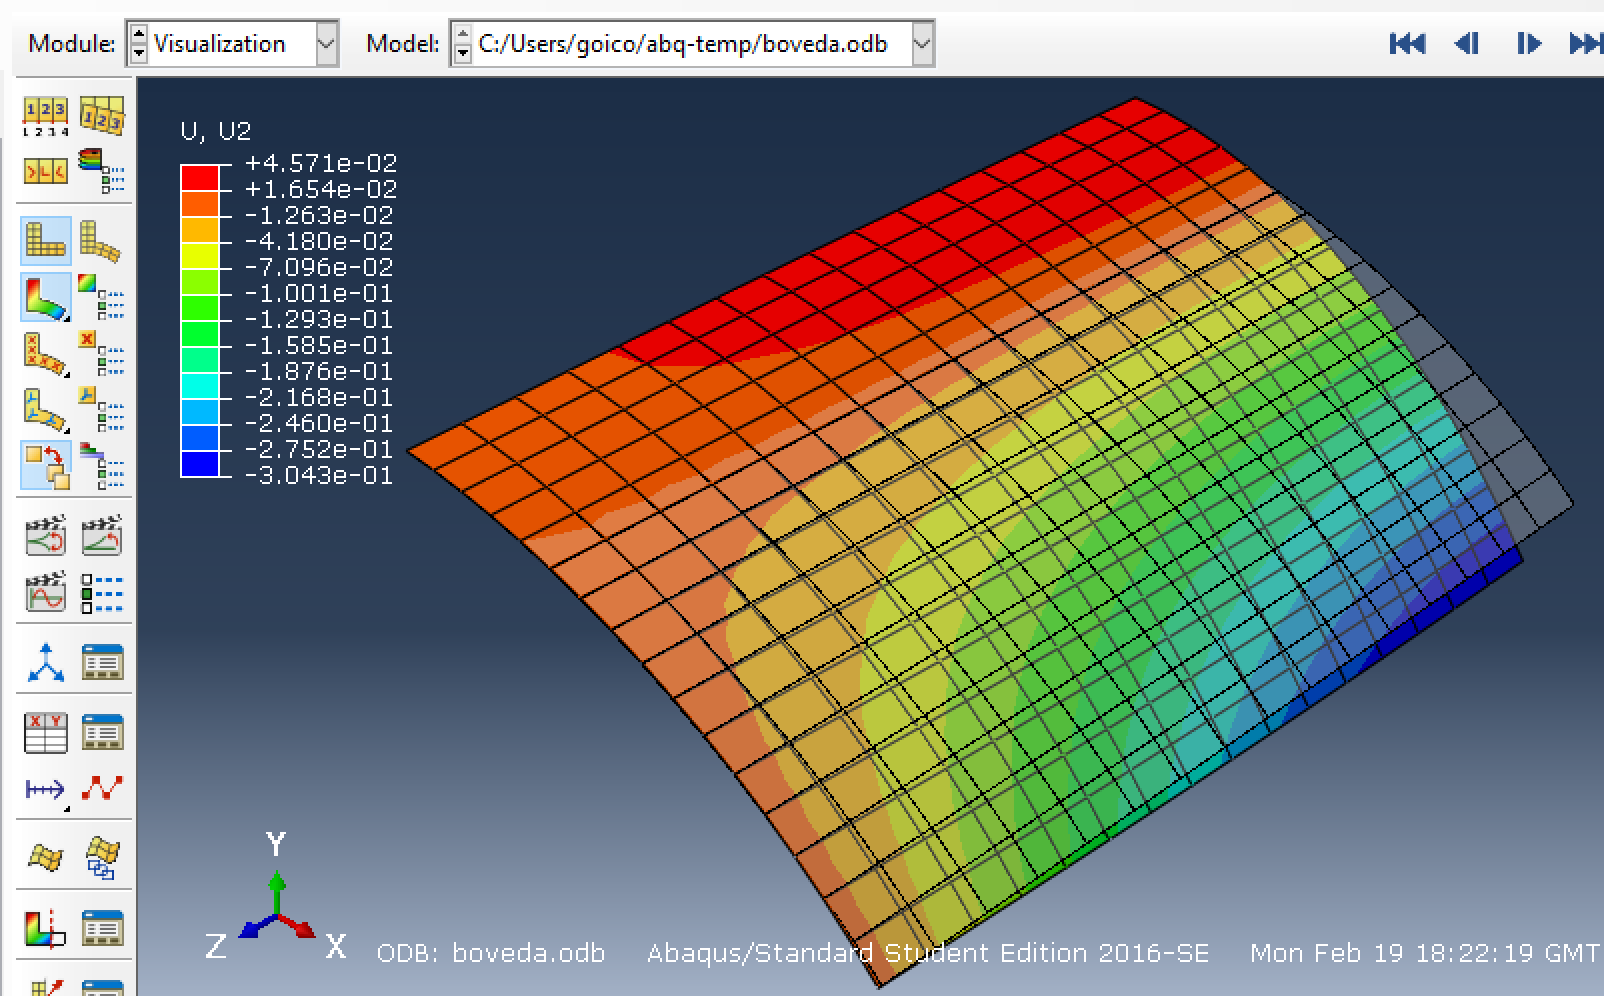
\includegraphics[scale=0.45]{capturas2019/a_fig23.png}
\caption{Resultados del cálculo -- desplazamiento vertical \texttt{U2}}
\label{fig:job-results}
\end{figure}
\begin{figure}[h!tp]
\centering
%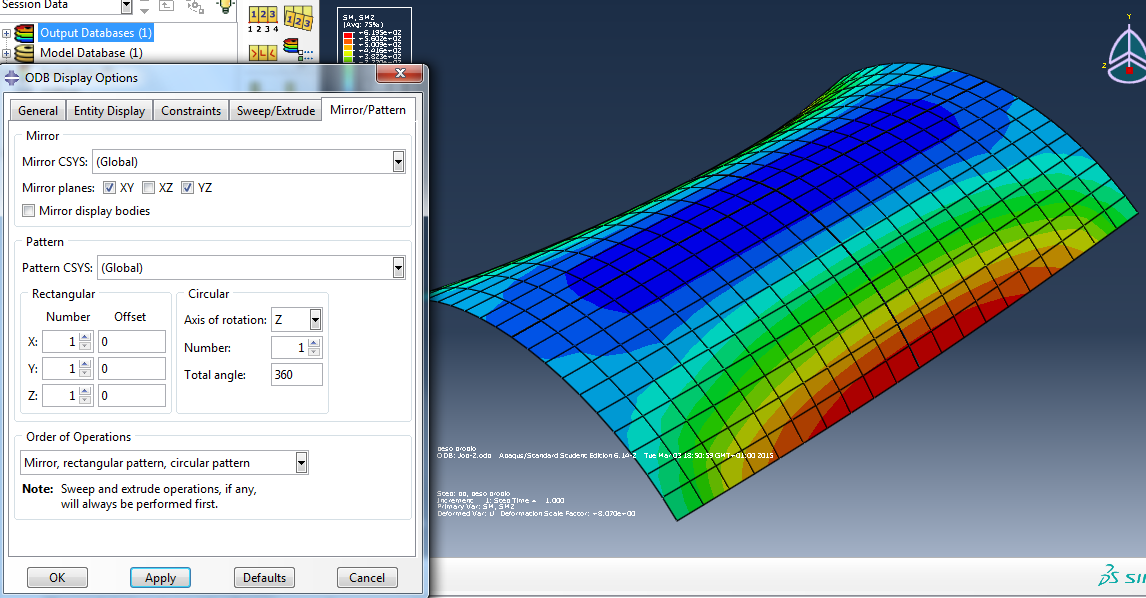
\includegraphics[scale=0.4]{capturas/39a-results.png}
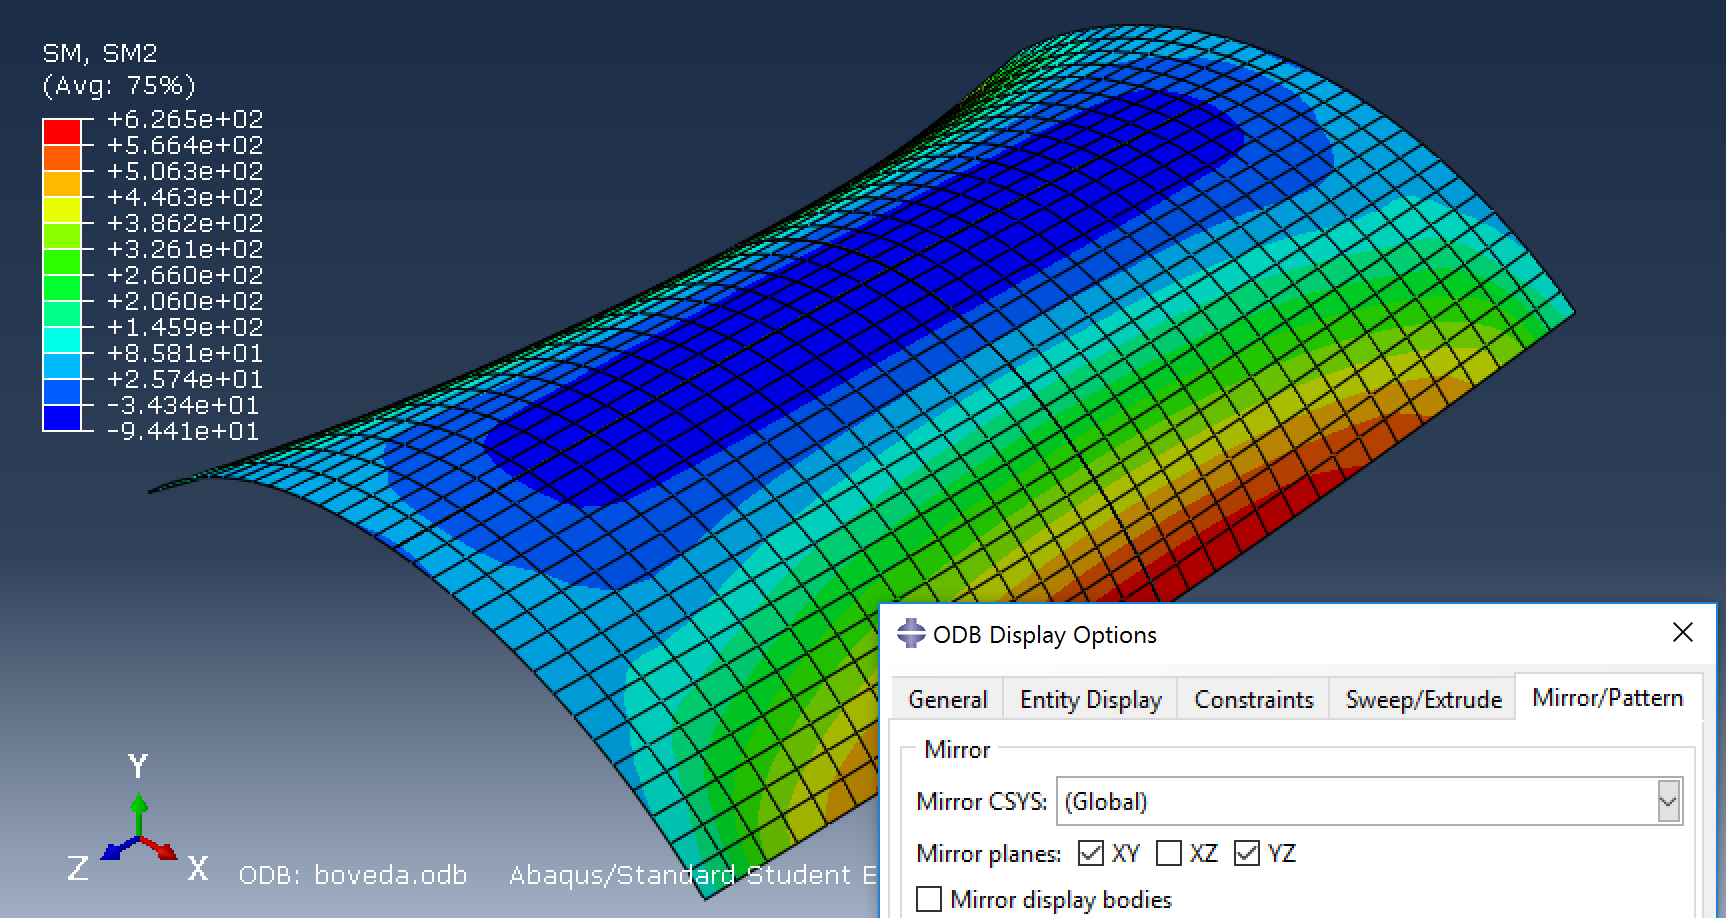
\includegraphics[scale=0.45]{capturas2019/a_fig24p.png}
\caption{Vista del modelo completo con las partes simétricas representadas}
\label{fig:job-results-symm}
\end{figure}
\clearpage

\section{Modelo con elementos de continuo}
Se puede crear un modelo similar con elementos de continuo (sólidos 3D), siguiendo los siguientes pasos:
\paragraph{\S1.---}
Crear una parte del tipo ``Deformable'' / ``Solid'' / ``Extrusion'';
Definir el contorno de la parte mediante dos arcos de circunferencia, con radios respectivos $R_{i}=R-e/2$ y $R_{e}=R+e/2$, con los mismos $40^{\circ}$ que antes, y unir posteriormente los extremos de dichos arcos para formar un recinto cerrado en el plano $XY$.
Terminar y extruir dicho perfil la distancia $L/2=25$ para obtener la geometría 3D de la parte, figura \ref{fig:part-solid}.
\begin{figure}[h!tp]
\centering
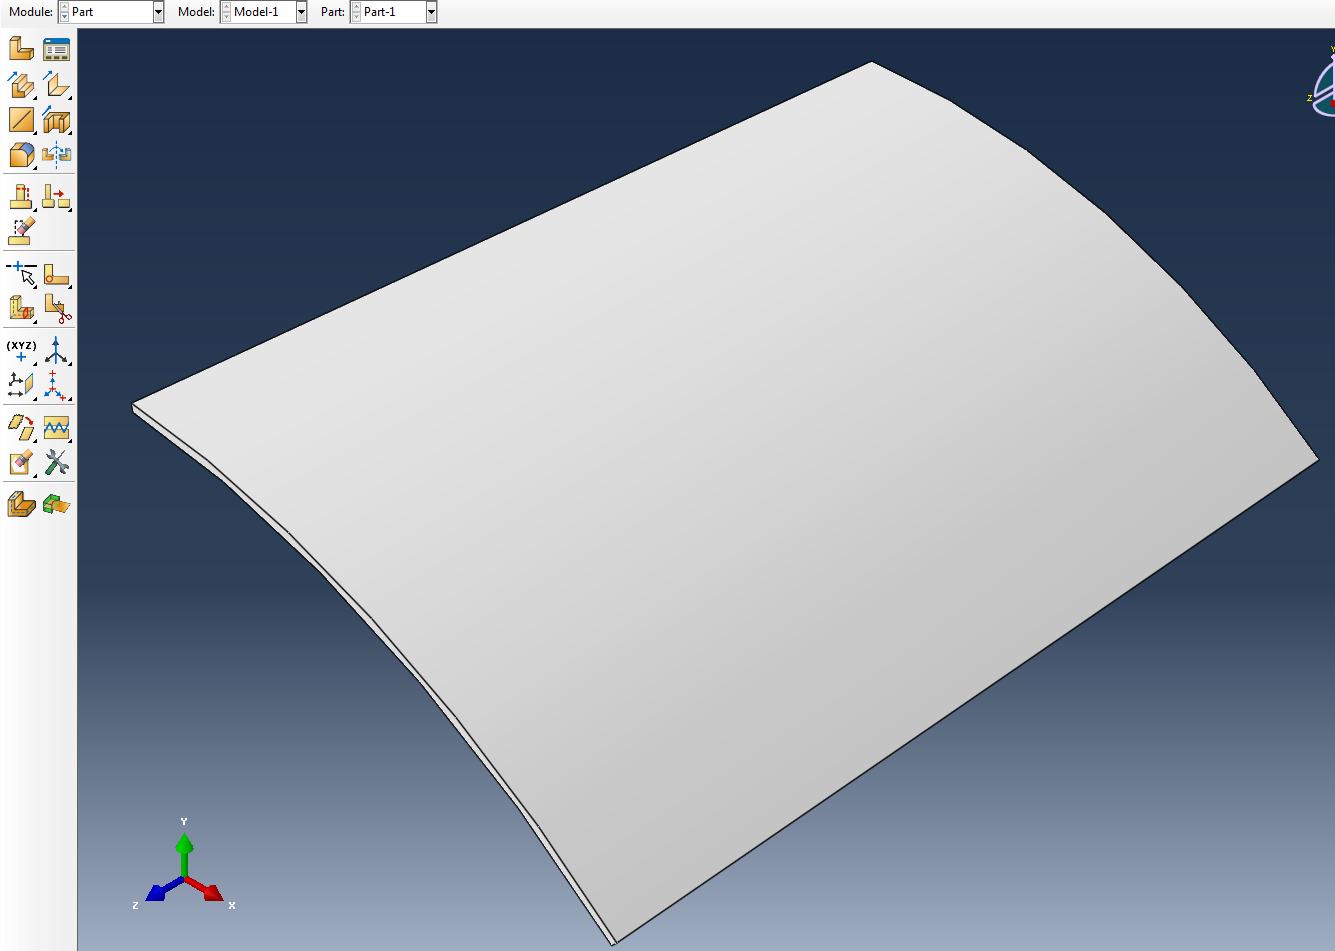
\includegraphics[scale=0.3]{capturas/40-part-solid.png}
\caption{Geometría de la parte como continuo 3D}
\label{fig:part-solid}
\end{figure}
\paragraph{\S2.---}
Para definir las condiciones de contorno en los bordes se debe tener cuidado de seleccionar el borde completo, no solo una arista, ver por ejemplo la figura \ref{fig:load-solid} en la que se definen las condiciones de simetría ``ZSYMM''.
El resto de condiciones de contorno en el modelo se establecen de forma similar.
\begin{figure}[h!tp]
\centering
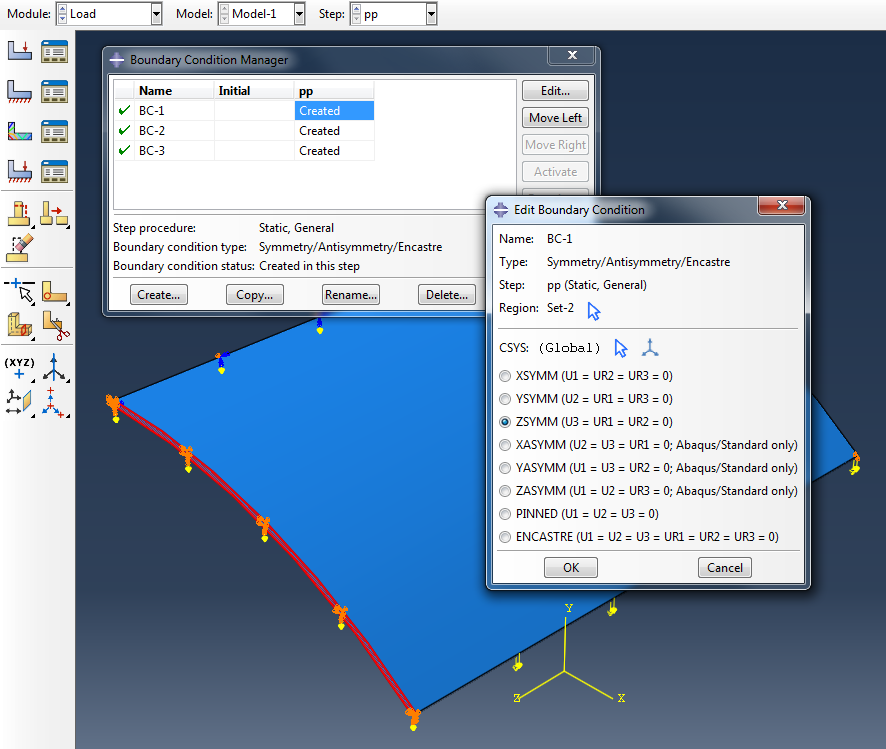
\includegraphics[scale=0.3]{capturas/41-load-solid.png}
\caption{Condiciones de contorno en modelo continuo 3D}
\label{fig:load-solid}
\end{figure}
\paragraph{\S3.---}
Para la selección del mallado en ``Mesh/controls'' adoptar una malla estructurada de Hexaedros, 
figura \ref{fig:mesh-c-solid}.
\paragraph{\S4.---}
En el tipo de elemento seleccionamos en primer lugar el hexaedro de modos incompatibles, se trata de un elemento especial que contiene grados de libertad adicionales para el campo de deformaciones, y que da buenos resultados para flexión a pesar de haber un solo elemento en el espesor,
figura \ref{fig:mesh-e-solid}.
\paragraph{\S5.---}
Para el mallado, basta con seleccionar las semillas que el sistema propone por defecto,
figura \ref{fig:mesh-s-solid}. 
El resultado obtenido, con un elemento solo en el espesor de la lámina, se muestra en la
figura \ref{fig:mesh-m-solid}. 
\begin{figure}[h!tp]
\parbox[t]{0.39\textwidth}{%
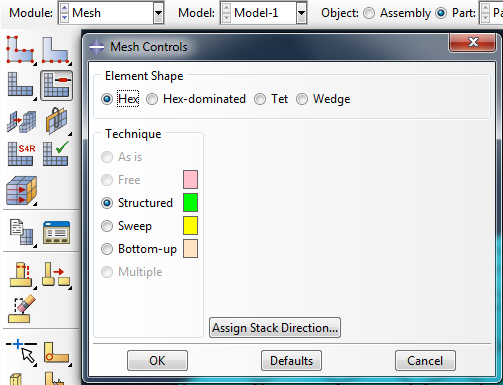
\includegraphics[width=\linewidth]{capturas/42-mesh-solid.png}
%\caption{``Mesh / controls'' in continuum 3D model}
\caption{``Mesh / controls'' en modelo continuo 3D}
\label{fig:mesh-c-solid}
}\quad
\parbox[t]{0.59\textwidth}{%
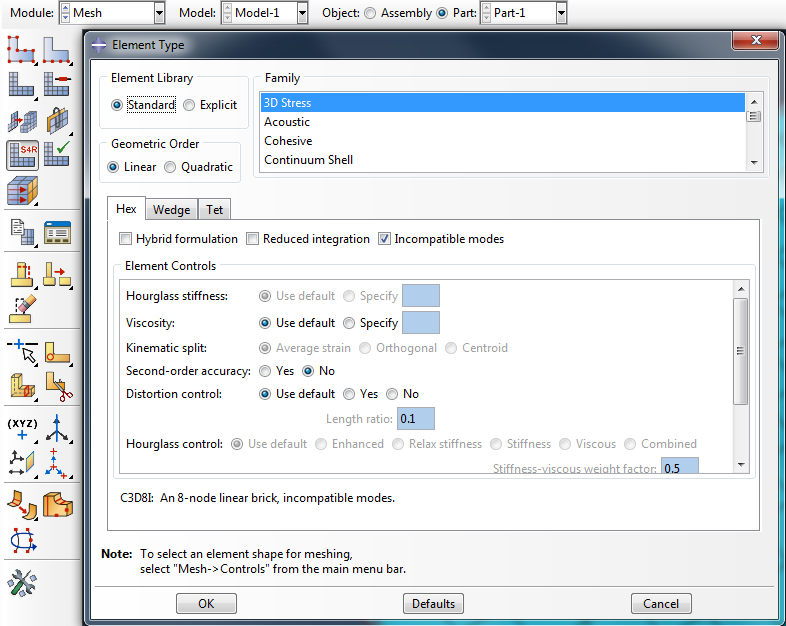
\includegraphics[width=\linewidth]{capturas/43-mesh-solid.png}
%\caption{Selection of element type (8 node hexahedron with incompatible modes) within ``Mesh / element type'' for the continuum 3D model}
\caption{Selección del tipo de elemento (hexaedro de 8 nodos con modos incompatibles) mediante ``Mesh / element type'' en modelo continuo 3D}
\label{fig:mesh-e-solid}
}%
\end{figure}
\begin{figure}[htp]
\centering
\includegraphics[scale=0.5]{capturas/44-mesh-solid.png}
\caption{Semillas para el mallado en modelo continuo 3D}
\label{fig:mesh-s-solid}
\end{figure}
\begin{figure}[htb]
\centering
\includegraphics[scale=0.45]{capturas/45-mesh-solid.png}
\caption{Malla de hexaedros en el modelo continuo 3D}
\label{fig:mesh-m-solid}
\end{figure}

Los resultados obtenidos con los elementos C3D8I son excelentes, muy similares a los de elementos lámina. La muestra más significativa es la flecha en el centro del borde libre, que resulta ser muy cercana al valor de referencia $u_{z}=-0.3024$ m.
% en este modelo con 14x19x1 elementos resulta $u_{z}=-0.3032$ m.

Si se modifica el tipo de elemento por el hexaedro lineal estándar con integración completa (C3D8) los resultados son extremadamente malos, la flecha resulta $u_{z}=-0.072$ m.
Por último, empleando el elemento hexaedro lineal con integración reducida (C3D8R) los resultados son también muy malos, aunque no tanto como en el caso anterior, la flecha resulta $u_{z}=-0.210\,\text{m}$.
Esto era de esperar ya que con la formulación normal de elementos no es posible representar el gradiente de desplazamientos debido a la flexión si se emplea solo un elemento en el espesor. Como mínimo serían necesario 4 ó 5 elementos en el espesor, pero esto conduciría a un modelo con un número muy elevado de grados de libertad y muy costoso.
El caso de los elementos con modos incompatibles es una excepción, en su formulación incluyen campos de deformaciones independientes que se adaptan y recogen correctamente las deformaciones de flexión. 

\clearpage

\section{Generación de modelos con scripts \texttt{Python}}

\subsection{Modelo con elementos lámina}

Se incluyen dos modelos preparados directamente en python que reproducen los modelos realizados con ayuda de abaqus cae.
En lo que sigue se explican someramente las distintas partes de cada script.

El primer modelo es el preparado para elementos lámina.
Se puede descargar directamente en \href{http://stokes.mecanica.upm.es/MCIC_open/practicas/scripts-python/prac3_lamina1.py}{\ttfamily prac3\_lamina1.py}, una vez descargado se puede ejecutar desde abaqus directamente.

En este modelo las fases seguidas en la programación son las siguientes, describiéndose los puntos en el croquis de la figura \ref{fig:lamina1}.
\begin{figure}
\centering
%    \includegraphics[width=1.0\textwidth]{imag/im5}
	\includegraphics[scale=0.25]{figs/prac3_lamina1_fig.png}
%  \caption{Nodes and selection}
	\caption{Croquis para generación de modelo con \texttt{Python} y elementos lámina}
	\label{fig:lamina1}
\end{figure}

\begin{enumerate}
\item
Primeramente se define el perfil de la lámina. Esto se hace ayudándose de los puntos que definen el cuarto de lámina que se va a modelar.
Estos son, el punto $O$ centro de la circunferencia que define la sección transversal de la lámina, $A$ que es el punto de máxima altura de la lámina y que 
pertenece al plano de simetría longitudinal de la misma y el punto $B$ que pertenece al borde libre. Adicionalmente se define el punto $M$ que se utilizará 
más adelante.
También se definen como variables de python el radio de curvatura de la lámina y el semiángulo (R y ANG).
\item
Con estos parámetros se definen los puntos en un sistema de coordenadas de dos dimensiones, se crea el arco de circunferencia que
define el perfil de la lámina y se realiza la extrusión que genera una parte (p).
\item
A continuación se definen el material, la sección (en terminología de abaqus) y la asignación de sección a parte.
Obsérvese que para hacer la asignación se usan las  'faces' de la parte de abaqus que representan la superficie ya generada.
\item
Una vez definido el material y asignado a la parte se genera la instancia a calcular que se denominará 'laminainstancia' y que se almacena en la 
variable 'myAssembly'. Aquí al generar la instancia se define con malla dependiente de la parte (dependent=ON).
\item
Posteriormente se definen las cargas y condiciones de contorno.
Para seleccionar los elementos geométricos en los que definir las condiciones de contorno nos apoyamos en los puntos medios de los bordes.
Con estos puntos medios buscamos el elemento geométrico al que aplica la condición de contorno. En este caso son elementos geométricos del tipo 'edges'. Para
esta búsqueda utilizamos puntos definidos en un espacio de tres dimensiones por lo que del punto $M$ definido inicialmente se usan sus dos coordenadas suplementadas
por la coordenada $z$ lo que da lugar al punto $OM3$.
Para definir el peso propio hay que seleccionar toda la instancia lo que se hace a  mediante un `BoundingBox` de `faces`.
\item
Para definir la malla se generan las divisiones de elementos en dos bordes de la lámina no paralelos, se define el tipo de elemento y se genera la malla.
\item
Por último se ejecuta el modelo y se almacena la definición del mismo.
\end{enumerate}

\subsection{Modelo con elementos de continuo}

El script del modelo con elementos de continuo se puede descargar en \href{http://stokes.mecanica.upm.es/MCIC_open/practicas/scripts-python/prac3_lamina2.py}{\ttfamily prac3\_lamina2.py}. 
Una vez descargado se puede ejecutar desde abaqus directamente.

La programación del script sigue las mismas pautas, con las salvedades correspondientes. 
Se describen los puntos en el croquis de la figura \ref{fig:lamina2}.
\begin{figure}
\centering
%    \includegraphics[width=1.0\textwidth]{imag/im5}
	\includegraphics[scale=0.25]{figs/prac3_lamina2_fig.png}
%  \caption{Nodes and selection}
	\caption{Croquis para generación de modelo con \texttt{Python} y elementos de continuo}
	\label{fig:lamina2}
\end{figure}
\begin{enumerate}
\item
Ahora se genera una sección que en vez de estar definida por un 
tramo de curva abierta se define con una curva cerrada.
Los puntos se definen con el siguiente criterio, los puntos pertenecientes a la parte superior de la lámina llevan el sufijo $T$ y los correspondientes
a la parte inferior el sufijo $B$.
\item
La parte se crea mediante una extrusión sólida, BaseSolidExtrude, como contraposición a la lámina que era  BaseShellExtrude.
\item
La definición del material es similar pero algo más sencilla que en la lámina.
\item
La definición de las cargas se hace utilizando igual que antes puntos medios pero que en este caso en vez de pertenecer a un borde (edge) pertenecen a una 
superficie (face). El procedimiento es el mismo que antes, se define el punto medio de la superficie a la que hay que asociar la condición de contorno y se 
busca la 'face' de la instancia mediante ' findAt'.
Para el peso propio se selecciona toda la instancia y para la condición de apoyo se selecciona sólo un borde, en este caso el inferior.
\item
La generación de malla en este caso es con una semilla para todo el modelo.
\item
El resto del script es similar.
\end{enumerate}


\section{Resultados}
\label{sec:resultados}
\subsection{Flecha en un nodo}

\paragraph{Paso 1.} Se trata de obtener la flecha en el punto medio del borde libre, que para el modelo de referencia es $u_{z}=-0.3024$ m.
\begin{figure}[h!tp]
%\begin{center}
%	\subfigure[Tools, query]{\includegraphics[width=0.6\textwidth]{imag/im2_a}}\quad
%	\subfigure[Probe values]{\includegraphics[width=0.25\textwidth]{imag/im3}}
\centering
	\subfigure[Tools, query]{\includegraphics[scale=0.50]{capturas2019/a_fig31a.png}}\quad
	\subfigure[Probe values]{\includegraphics[scale=0.50]{capturas2019/a_fig31b.png}}
%\end{center}
\caption{Seleccionar valores a mostrar de los resultados}
\label{fig2a}
\end{figure}

Se procede utilizando el menú de tools (dentro de resultados) y dentro de tools el submenú query (Fig.~\ref{fig2a}(a)). Al optar por este submenú 
se abre un recuadro en el que se debe elegir la opción ``Probe values'' (\emph{sondear valores}), 
Fig.~\ref{fig2a}(b).
Aparece una nueva ventana en la que se debe elegir ``Probe: Nodes'' y ``Components: Selected'' (Fig.~\ref{fig5}). En la cabecera de esta ventana aparece el campo que se está visualizando que será el que se sondee: \emph{Field output variable for Probe:}
U, U2, que se puede seleccionar mediante el icono al comienzo de este campo, Fig.~\ref{fig7}.
\begin{figure}[h!tp]
\centering
%    \includegraphics[width=1.0\textwidth]{imag/im5}
	\includegraphics[scale=0.45]{capturas2019/a_fig32.png}
%  \caption{Nodes and selection}
	\caption{Nodos y selección}
	\label{fig5}
\end{figure}
\begin{figure}[h!tp]
\centering
%	\includegraphics[width=0.75\textwidth]{imag/im7}
	\includegraphics[scale=0.45]{capturas2019/a_fig33.png}
	\caption{Selección de variable a sondear (\emph{probe}): U, U2}
	\label{fig7}
\end{figure}

Una vez seleccionados esos campos se debe marcar con el ratón en la ventana de representación del modelo el o los nodos en los que estamos interesados.
Al hacer clic con el ratón sobre el nodo en cuestión se verá el resultado en la ventana de \emph{Probe Values} que resulta ser $u_{z}=-0.3043$ m, lo que coincide con el valor esperado (Fig.~\ref{fig8}). 
%(Nota: esta malla de $7\times 10$ es más grosera que la pedida en el ejercicio ($16\times 16$, por lo que el valor resulta ligeramente distinto, algo menos preciso.)
\begin{figure}[h!tp]
\centering
%	\includegraphics[width=0.95\textwidth]{fm/Fig-1_Despla_Vertical.png}
	\includegraphics[scale=0.45]{capturas2019/a_fig34.png}
%	\includegraphics[width=0.8\textwidth]{imag/im8}
\caption{Valor de flecha (U2) en el nodo seleccionado}
\label{fig8}
\end{figure}

\clearpage

\subsection{Reacción en un borde}

Es también interesante obtener las reacciones en los apoyos o en los bordes que representan las condiciones de simetría.
Para ello se procede como en la práctica anterior. Se define una curva sobre el modelo, en este caso se tratará del borde en el que estemos interesados.
En la definición de la curva, al tratarse de bordes curvos (en general) se deberán incluir todos los nodos que la forman. 
Una vez definida la curva se define una tabla de datos mediante la asociación de un valor escalar a la curva predefinida.
En este caso particular se procedería del siguiente modo:
\begin{enumerate}
\item Se define la curva (\emph{path}) (Fig.~\ref{fig11}). 
Ello se hace a partir del árbol de resultados que figura en la 
ventana izquierda. 
Se selecciona ``\emph{Create}'' haciendo clic con el botón derecho del ratón sobre el item ``\emph{Paths}''.
\begin{figure}[h!tp]
\centering
%	\includegraphics[width=0.8\textwidth]{imag/im11}
	\includegraphics[scale=0.45]{capturas2019/a_fig35.png}
%	\includegraphics[scale=0.45]{capturas2019/a_fig35p_fig36a.png}
\caption{Creación de una curva (\emph{path})}
\label{fig11}
\end{figure}

En la ventana siguiente (Fig.~\ref{fig13}(a)) se selecciona ``Node list'', se da un nombre a la curva y se hace clic sobre ``continue''.
En la siguiente ventana (Fig.~\ref{fig13}(b)) se indica ``Add After'' para la creación del ``Node List''.
\begin{figure}[!htp]
\centering
%    \subfigure[Tipo de curva]{\includegraphics[scale=0.55]{imag/im13}}
%    \subfigure[Node List]{\includegraphics[scale=0.55]{imag/im14}}
	\subfigure[Tipo de curva]{\includegraphics[scale=0.45]{capturas2019/a_fig36a.png}}
	\quad
	\subfigure[Node List]{\includegraphics[scale=0.45]{capturas2019/a_fig36b.png}}
\caption{Tipo de curva y lista de nodos para definición del \emph{Path}}
\label{fig13}
\end{figure}

Se van añadiendo los nodos hasta que una vez añadidos todos se hace clic sobre ``Done'', como se muestra en la figura~\ref{fig19}.
Se confirma y ya está creada la curva, como se puede observar en el árbol que representa los resultados.
\begin{figure}[h!tp]
\centering
%	\includegraphics[width=0.9\textwidth]{fm/Fig-2_Reacc_Vertical.png}
	\includegraphics[scale=0.45]{capturas2019/a_fig37-2.png}
\caption{\emph{Path} para la Reacción Vertical}
\label{fig19}
\end{figure}

\clearpage

\item El siguiente paso es asociar un resultado a la curva, para lo cual se crea una tabla, de modo similar 
a la creación de la curva. Se hace clic sobre el apartado ``XYData'' del árbol (Fig.~\ref{fig21}).
\begin{figure}[h!tp]
\centering
%    \includegraphics[width=0.9\textwidth]{imag/im21}
	\includegraphics[scale=0.45]{capturas2019/a_fig38.png}
\caption{Creación de una tabla de datos}
\label{fig21}
\end{figure}

En la siguiente ventana (fig.~\ref{fig22}(b)) se elige la opción ``Path'' y se continúa.
Después (Fig.~\ref{fig22}(b)) se asocia a la curva indicada en el menú desplegable de ``Path'' el valor del escalar que nos interese. 
\begin{figure}[h!tp]
\centering
%    \subfigure[\emph{Source}]{\includegraphics[scale=0.45]{imag/im22}}
%    \subfigure[\emph{Data Extraction}]{\includegraphics[scale=0.45]{imag/im24}}
	\subfigure[\emph{Source}]{\includegraphics[scale=0.45]{capturas2019/a_fig39a.png}}
	\quad
	\subfigure[\emph{Data Extraction}]{\includegraphics[scale=0.45]{capturas2019/a_fig39pb.png}}
\caption{Definición de la trayectoria (\emph{path}) para una curva de resultados}
\label{fig22}
\end{figure}
Para ``X Values'' dejamos la opción de \emph{``True distance''} y en ``Data Extraction'', aparte de elegir la curva, marcamos \emph{``Undeformed''} e \emph{``Include intersections''}. 
Para el valor de la ordenada de la curva se hace clic sobre el botón ``Field Output'' con lo que tendremos acceso a la ventana 
de la fig.~\ref{fig26}(a), en la que elegiremos RF, RF2 y haremos clic sobre ``OK''. Ya sólo queda marcar ``Plot''
en la ventana de Data Extraction (Fig.~\ref{fig26}(b)) con lo que obtendremos la curva de la figura fig.~\ref{fig28}.
\begin{figure}[h!tp]
\centering
%    \subfigure[Componente RF2]{\includegraphics[scale=0.45]{imag/im26}}\quad
%    \subfigure[\emph{Data Extraction}: opciones]{\includegraphics[scale=0.45]{imag/im27}}
	\subfigure[Componente RF2]{\includegraphics[scale=0.45]{capturas2019/a_fig40pa.png}}
	\quad
	\subfigure[\emph{Data Extraction}: opciones]{\includegraphics[scale=0.45]{capturas2019/a_fig40pb.png}}
\caption{Extracción de datos a una tabla}
\label{fig26}
\end{figure}
\begin{figure}[!htp]
\centering
%\includegraphics[width=0.9\textwidth]{fm/Fig-3_Reacc_Vertical_longitud.png}
\includegraphics[scale=0.35]{capturas2019/a_fig41p2a.png}
\quad
\includegraphics[scale=0.35]{capturas2019/a_fig41p2.png}
\caption{Reacción vertical por unidad de longitud en apoyo}
  \label{fig28}
\end{figure}
\end{enumerate}
Además, se puede obtener la integral de la reacción por unidad de longitud, mediante la selección en el árbol del modelo
\emph{XY Data} $\to$ \emph{Create} $\to$ \emph{Operate on XY data} $\to$ \emph{integrate}
obteniendo el resultado de la figura~\ref{fig:int-reac-vert}.
\begin{figure}[!htbp]
\centering
%\includegraphics[width=0.9\textwidth]{fm/Fig-4_Integral_Reacc_Vertical}
\includegraphics[scale=0.45]{capturas2019/a_fig42p.png}
\caption{Integral de la reacción vertical (\emph{Moment} representa la integral)}
\label{fig:int-reac-vert}
\end{figure}
%\clearpage

Es interesante hacer como comprobación los cálculos directos de la reacción total, figura~\ref{fig:calc-anal-reac}, que comprobamos que difiere ligeramente (5\%) del valor integrado en el \emph{path}.
La razón es que la opción \emph{path} no es la forma más exacta de sumar reacciones ya que hay una interpolación de por medio. 
La forma más precisa sería sumar las reacciones individuales de cada uno de los nodos, como se aprecia en la figura~\ref{fig:suma-reac-nod}
\begin{figure}[!htbp]
\centering
\includegraphics{fm/Fig-5_Analitico_Reacc_Vertical}
\caption{Cálculo analítico de la reacción}
\label{fig:calc-anal-reac}
\end{figure}
\begin{figure}[!htbp]
\centering
%\includegraphics[scale=0.8]{fm/Fig-6_Suma_reacciones.png}
\includegraphics[scale=0.45]{capturas2019/a_fig44p1.png}
\caption{Suma de reacciones nodales}
\label{fig:suma-reac-nod}
\end{figure}

Otra forma de obtener la suma de reacciones sin tener que \emph{sumarlas manualmente} es establecer una restricción de todos los nodos  del borde de interés a un único nodo mediante un \emph{MPC} o un \emph{kinematic coupling} y recuperar la reacción en dicho nodo.
Para ello al borde anterior se acopla una restricción cinemática a un único nodo que puede ser real o ficticio y al que se asigna la condición de contorno fija. 
De este modo la reacción obtenida es la correspondiente a la resultante total de ese borde. 
En este caso el nodo maestro es uno de los vértices, figura~\ref{fig:asig-kine-coup}.
\begin{figure}[!htp]
\centering
\includegraphics[width=0.9\textwidth]{fm/Fig-7_Kinematic_constraint.png}
\caption{Asignación de \emph{kinematic coupling} MPC}
\label{fig:asig-kine-coup}
\end{figure}

Se asigna la condición de contorno al nodo maestro, figura~\ref{fig:asig-cond-cont}.
\begin{figure}[!htp]
\centering
\includegraphics[width=0.9\textwidth]{fm/Fig-8_BC_Nodo_Maestro.png}
\caption{Asignación condición de contorno}
\label{fig:asig-cond-cont}
\end{figure}

Si se hace así el resultado es completamente exacto como se puede apreciar en la figura~\ref{fig:calc-reak-kinem}.
\begin{figure}[!htp]
\centering
\includegraphics[width=0.9\textwidth]{fm/Fig-9_Kinematic_Reacc_Vertical.png}
\caption{Cálculo de la reacción mediante \emph{kinematic coupling}}
\label{fig:calc-reak-kinem}
\end{figure}
%\clearpage
\addtocontents{toc}{\protect\vspace{1ex} \protect\hrule}
\mbox{}

\clearpage
\section{Ejercicio propuesto}
El puente de la Fig.~\ref{figuprop1}, de ancho 3,5 m, se encuentra empotrado en pilas y estribos en las áreas verticales de contacto con el terreno circundante. El módulo de Young del material es de 30.0 GPa, el coeficiente de Poisson es $\nu=0.2$ y el peso específico es $\gamma=24000 \mathrm{~N} / \mathrm{m}^{3}$. Las acciones a considerar serán el peso propio y el efecto de un sismo que se supondrá equivalente a una fuerza volumétrica, distribuida transversalmente al puente, de valor $1000 \mathrm{~N} / \mathrm{m}^{3}$, actuando en el sentido AB (Fig.~\ref{figuprop1}).

Se desea estudiar el comportamiento estructural de este puente ante las dos acciones mencionadas. Teniendo en cuenta las simetrías del problema, se preparará un modelo con Abaqus de la mitad del puente tal y como se indica en la Fig.~\ref{figuprop1}, donde se detalla la geometría de la estructura.

\begin{figure}[!h]
  \begin{center}
    \includegraphics[width=0.55\textwidth]{./figs/prop}
  \end{center}
  \caption{Descripción del ejercicio propuesto}
  \label{figuprop1}
\end{figure}

Responde las preguntas que vienen a continuación teniendo en cuenta que el elemento a emplear será el hexaedro de 8 nodos con integración reducida C3D8R y el tamaño del elemento a utilizar en el mallador de Abaqus será $0.55 \mathrm{~m}$.

\begin{enumerate}
\item Flecha vertical (valor absoluto) en el punto B:
  \begin{multicols}{4}
  \mybox{A: $3.1\cdot 10^{-5}$ $m$} 
\columnbreak
\mybox{B: $42.1\cdot 10^{-3}$ $m$}
\columnbreak
\mybox{C: $42.1\cdot 10^{-5}$ $m$} %ok$
\columnbreak
\mybox{D: $3.1\cdot 10^{-3}$ $m$}
  \end{multicols}
\item Peso total del modelo:
  \begin{multicols}{4}
\mybox{A: 0.0679 MN}
\columnbreak
\mybox{B: 0.8148 MN} 
\columnbreak
\mybox{C: 1.0 MN}
\columnbreak
\mybox{D: 1.6296 MN} %ok$
  \end{multicols}
\item M\'axima tensi\'on de tracci\'on en el modelo:
  \begin{multicols}{4}
\mybox{A:  $0.09$ MPa}
\columnbreak
\mybox{B: $-1.642$ MPa} 
\columnbreak
\mybox{C: $0.393$ MPa}%ok$
\columnbreak
\mybox{D: $450.6$ MPa}
\end{multicols}
\item Suma de las reacciones horizontales (direcci\'on AB) del modelo en valor absoluto:
  \begin{multicols}{4}
\mybox{A:  $1629.6$ kN}
\columnbreak
\mybox{B:  $1.0$ kN} 
\columnbreak
\mybox{C: $67.9$ kN}%ok$
\columnbreak
\mybox{D: $0.5$ kN}
\end{multicols}
\item M\'inima tensi\'on de compresi\'on en el centroide del elemento E1:
  \begin{multicols}{4}
\mybox{A:   $-0.113$ MPa}
\columnbreak
\mybox{B: $0.5$ MPa} 
\columnbreak
\mybox{C: $-1.47$ MPa}%ok$
\columnbreak
\mybox{D:  $0.113$ MPa}
\end{multicols}
\item Tensi\'on vertical en el punto D:
  \begin{multicols}{4}
\mybox{A:  $-283.5$ kPa}%ok$
\columnbreak
\mybox{B:  $-3048.4$ kPa} 
\columnbreak
\mybox{C:  $-30.9$ kPa}
\columnbreak
\mybox{D:   $117.9$ kPa}
\end{multicols}
\end{enumerate}

\end{document}
